\documentclass[16pts]{report}

\usepackage[utf8]{inputenc}
\usepackage[T1]{fontenc}
\usepackage[francais]{babel}
\usepackage{xcolor}
\usepackage[hyphens]{url}
\usepackage[hidelinks]{hyperref}
\usepackage{amsmath}
\usepackage{graphicx}
\usepackage{geometry}
\usepackage{textcomp}
\usepackage{tabularx}
\usepackage{wrapfig}
\usepackage{lscape}
\usepackage{rotating}

\usepackage{titlesec}
\setcounter{secnumdepth}{4}
\titleformat{\paragraph} {\normalfont\normalsize\bfseries}{\theparagraph}{1em}{}
\titlespacing*{\paragraph} {0pt}{3.25ex plus 1ex minus .2ex}{1.5ex plus .2ex}

%\hypersetup{hypertexnames=true}
\geometry{hmargin=2.5cm,vmargin=1.5cm}

\usepackage{listings}
\lstdefinestyle{customc}{
  belowcaptionskip=1\baselineskip,
  breaklines=true,
  frame=L,
  xleftmargin=\parindent,
  language=python,
  showstringspaces=false,
  basicstyle=\footnotesize\ttfamily,
  keywordstyle=\bfseries\color{green!40!black},
  commentstyle=\itshape\color{purple!40!black},
  identifierstyle=\color{blue},
  stringstyle=\color{orange},
}
\lstset{escapechar=@,style=customc}
\usepackage{float} %Option H pour les figures, utile.

\title{Rapport du projet de PDP \\ Aide à la compilation d'un noyau Linux}
\author{Aupetit Jordan, Berarde Fabien, Lemasson Mickael, Thiao-Layel Bruno}

\usepackage{fancyhdr}
\pagestyle{fancy}
\usepackage{lastpage}


\fancypagestyle{IHA-fancy-style}{%
  \fancyhf{}% Clear header and footer
  \fancyhead[L]{Université de Bordeaux\\
  Projet de programmation : Aide à la compilation d'un noyau Linux}
  \fancyhead[CR]{}
  \fancyfoot[C]{\thepage/\pageref{LastPage}\\}% Custom footer
  \renewcommand{\headrulewidth}{1pt}
  \renewcommand{\footrulewidth}{1pt}
}

% Redefine the plain page style
\fancypagestyle{plain}{%
  \fancyhf{}%
  \fancyhead[L]{Université de Bordeaux\\
  Projet de programmation : Aide à la compilation d'un noyau Linux}
  \fancyhead[CR]{}
  \fancyfoot[C]{\thepage/\pageref{LastPage}\\}%
  \renewcommand{\headrulewidth}{1pt}
  \renewcommand{\footrulewidth}{1pt}
}

\fancypagestyle{test}{%
  \fancyhf{}%
  \fancyhead[L]{Université de Bordeaux\\
  Projet de programmation : Aide à la compilation d'un noyau Linux}
}

\begin{document}

\maketitle
\clearpage
Remerciements\\

Nous tenons à remercier toutes les personnes qui ont aidé au cours de notre
projet et en particulier :\\

\begin{itemize}
  \item Xavier Blanc, notre chargé de TD, pour sa disponibilité et ses conseils
      prodigués tout au long de notre projet, autant sur la phase d'analyse que
      sur la phase de développement.\\
  \item Xavier de Rochefort et Alan Charpentier, pour avoir toujours été
      disponible et avoir répondu à toutes nos questions concernant leurs
      attentes. \\
  \item Philippe Narbel, notre professeur de Projet de Programmation, pour tous
      les conseils qu'il nous a donné concernant la gestion de projet, la
      formalisation et la structuration du code.\\
  \item Le jury, pour le temps qu'il a accordé à la lecture de notre mémoire.\\
\end{itemize}
\pagestyle{test}
\tableofcontents
\clearpage
\bibliographystyle{unsrt}
\nocite{*}


\pagestyle{IHA-fancy-style}
Dans le cadre de notre projet de programmation de première année de Master,
nous avons choisi le sujet « Aide à la compilation de noyaux Linux ».  \\

Ce sujet consiste à créer un outil permettant de configurer un noyau répondant
uniquement aux besoins de l'utilisateur. Il est déjà possible de configurer
soi-même un noyau, mais la tâche peut être très fastidieuse à cause du manque
de simplicité des solutions proposées. La plus-value que nous allons apporter
sera de permettre à un utilisateur non expert de configurer simplement son
noyau en l'allégeant à sa guise.  \\

Dans ce mémoire, nous présentons, dans un premier temps, les objectifs de notre
projet, puis nous expliquons l’organisation aussi bien au niveau technique que
fonctionnelle de notre groupe. Ensuite nous analysons l'existant de ce projet.
\\

Puis, nous développons les aspects relatifs à l’analyse avec la définition des
différents besoins du client et à la conception ainsi que la réalisation de
notre projet et les tests réalisés.  \\

Enfin nous présentons les résultats obtenus ainsi que les perspectives, tant
fonctionnelles que techniques.


\chapter{Présentation du projet}
\label{cha:Présentation du projet}

Notre sujet « Aide à la compilation de noyaux Linux » a pour principal objectif
la conception d'un logiciel. Celui-ci doit permettre de pouvoir configurer un
noyau pour que l'utilisateur puisse avoir seulement les options qu'il souhaite.
Le fichier de configuration d'un noyau Linux est composé d'options qui
permettront lors de la compilation d'activer des services à la demande.
Certaines options requièrent ou excluent la présence d'autres options.  \\

Notre objectif premier est de créer un outil avec une interface simple et
accessible par un grand nombre d'utilisateurs. Nous ne devons pas perdre de vue
que la configuration d'un noyau est une tâche très longue et sujette aux
erreurs, de ce fait, une bonne ergonomie permettra de simplifier ce processus.
Nous devons également reprendre les fonctionnalités de base en permettant à
l'utilisateur de générer une configuration par défaut en fonction de
l'architecture qu'il choisit. Il doit pouvoir modifier les valeurs des options
qui ne sont pas en conflit et générer un fichier en fonction de ses choix.  \\

De plus, nous avons pour objectif de rajouter des fonctionnalités présentes
dans certaines des solutions existantes ou qui n'existent simplement pas.  Nous
avons dû permettre de faire une recherche d'option, non seulement sur son nom,
mais également sur sa description et son message d'aide.  \\

Ensuite, l'outil doit faciliter la résolution des conflits lorsque la valeur
d'une option n'est pas modifiable. En effet, il est possible qu'on ne puisse
pas activer une option, car celle-ci, par exemple, ne doit pas être activée en
même temps qu'une autre option. Nous affichons à l'utilisateur la liste des
options en conflit avec l'option qu'il souhaite activer pour qu'il puisse y
accéder rapidement.  \\

Enfin, en partant de l'idée de proposer une configuration par défaut en
fonction de son matériel, nous avons développé un site communautaire.  Celui-ci
est une base permettant d'ajouter, de modifier ou de supprimer des relations
entre un matériel et des options. Il sera alors possible de consulter cette
base afin de pouvoir trouver les options qui nous correspondent.  \\

\chapter{Organisation de l'équipe}
\label{cha:Organisation de l'équipe}
    \section{Fonctionnement de l'équipe}
    \label{sec:Fonctionnement de l'équipe}

Nous avions déjà décidé assez rapidement au début de l'année de Master de
former notre groupe pour le projet de programmation. Lors du choix des sujets,
nous avons pris en compte les préférences de chacun et nous avons ainsi pu
choisir ce sujet. Celui-ci nous a tout de suite intéressé puisque c'était avant
tout un projet concret qui vise à répondre à un réel besoin.  En ce qui
concerne la mise en place des bases de notre travail en équipe, nous avons
réussi à nous organiser rapidement.  \\

Dès le début, nous avons commencé à répartir nos tâches, ce qui nous a permis
d’avancer plus rapidement que ce soit dans l’analyse ou, plus tard, dans la
conception. Il était très important pour nous de bien les séparer, car malgré
un échange d’informations constant avec des outils tels que Git ou Google
Drive, il était parfois difficile de travailler à plusieurs sur une même tâche
sans se gêner mutuellement. Les sessions de travail individuelles étaient
souvent suivies de réunion, afin de rassembler les travaux de chacun.  \\


    \section{Gestion du projet}
    \label{sec:Gestion du projet}


    Au début du projet, nous avions établi un planning prévisionnel non
    schématisé des tâches à réaliser. Cependant, celui-ci a fait l'objet de
    diverses modifications en raison des différents aléas rencontrés.

    \begin{sidewaysfigure}
        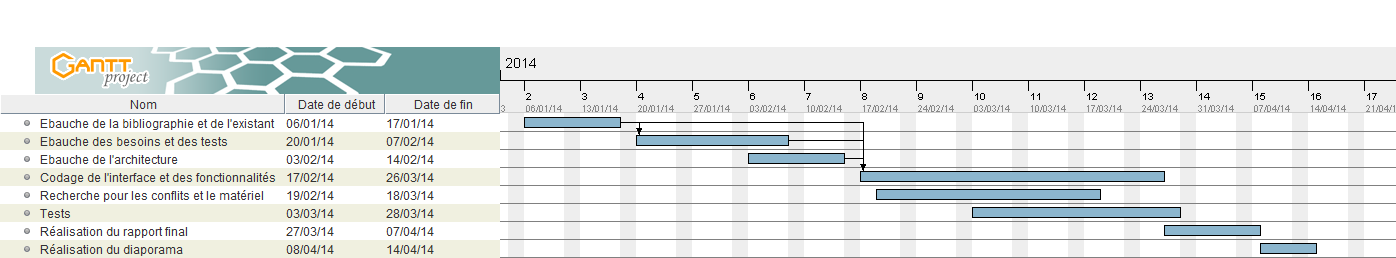
\includegraphics[scale=0.5]{./illustrations/planning_initial_pdp.png}
        \centering
        \caption{Planning initial du projet}
        \label{fig:PlanningInitial}
        \vspace{10.00mm}
        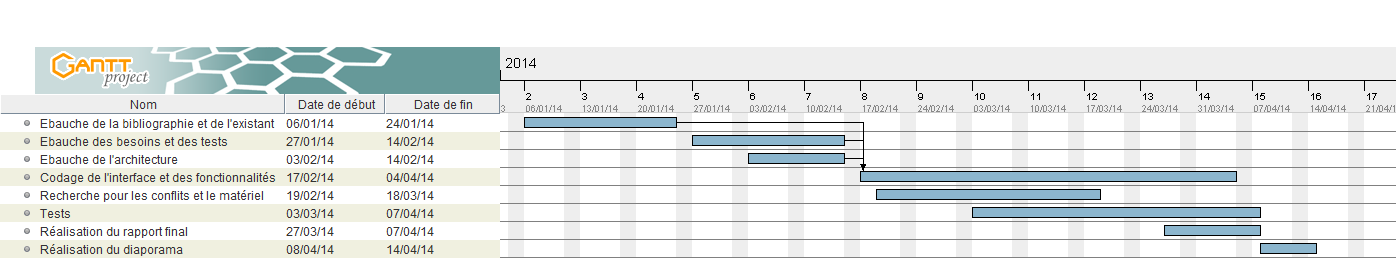
\includegraphics[scale=0.5]{./illustrations/planning_final_pdp.png}
        \centering
        \caption{Planning final du projet}
        \label{fig:PlanningFinal}
    \end{sidewaysfigure}

\newpage
Commentaires critiques\\

    Voici le planning prévisionnel de la réalisation de nos tâches durant notre
    projet ainsi que le planning final.  \\

    On peut constater que chaque tâche ne s'est pas déroulée comme prévu.  En
    effet, notre projet a nécessité une grande phase de recherche sur le
    problème de résolution des conflits, de détection du matériel et la
    réalisation des différents tests qui a duré plus longtemps.  Comme on peut
    le constater, la réalisation de l'ébauche de la bibliographie et de
    l'existant nous a pris une semaine supplémentaire suite aux retours que
    nous avions eu. Enfin, le codage de l'application et les tests se sont
    terminés avec un peu plus d'une semaine de retard par rapport à la date que
    nous avions prévu.  \\

    Ensuite, durant la phase de conception, nous avons pu modifier certaines
    tâches. En effet, la résolution des conflits a été écartée pour simplement
    aider l'utilisateur à trouver les options qui posent problème et en le
    laissant le corriger seul. L'idée de détecter automatiquement le matériel
    de l'utilisateur pour lui proposer une configuration a été abandonnée au
    profit d'un site communautaire contenant des relations entre des options et
    du matériel.


    \section{Logiciels et technologies utilisés}
    \label{sec:Logiciels et technologies utilisés}


\begin{figure}[H]
    
\includegraphics[scale=0.3]{illustrations/git.png} 
    
\includegraphics[scale=0.15]{illustrations/github.png} 
    \centering
\end{figure}

Git (1.9.0) est un logiciel de gestion de versions.  C'est un logiciel libre
créé par Linus Torvalds.  Git fonctionne de façon décentralisée, mais nous
utilisons les serveurs de Github pour gérer notre dépôt.  Nous avons utilisé ce
logiciel afin de faciliter le travail collaboratif. \\

\begin{figure}[H]
    
\includegraphics[scale=0.15]{illustrations/GoogleDrive.png} 
    \centering
\end{figure}

Google drive (1.14) est un service de stockage et de partage de fichiers 
dans le Cloud. Nous l'avons utilisé afin de pouvoir partager et éditer des documents 
de manière interactive.\\

\begin{figure}[H]
    
\includegraphics[scale=0.15]{illustrations/lucidchart.png} 
    \centering
\end{figure}

LucidChart est un service qui permet de travailler collaborativement à la 
réalisation de différents diagrammes. Nous nous sommes servis de celui-ci 
afin de réaliser les différents diagrammes relatifs à notre analyse.\\

\begin{figure}[H]
    
\includegraphics[scale=1.1]{illustrations/texmaker.png} 
    \centering
\end{figure}

Texmaker (4.1.1) est un logiciel libre destiné à l'édition de documents 
LaTeX. Il est possible de visionner le rendu de notre texte directement dans 
celui-ci. Nous l'avons utilisé afin de compiler nos fichiers LaTeX en PDF.\\

\begin{figure}[H]
    
\includegraphics[scale=0.2]{illustrations/python.png} 
    \centering
\end{figure}

Python (2.7.6) est un langage de programmation objet multiplateforme. 
Il favorise la programmation impérative structurée et orientée objet. Il 
est doté d'un typage dynamique fort, d'une gestion automatique de la 
mémoire par ramasse-miettes. Il est similaire au Perl, Ruby et Smalltalk. 
Nous avons décidé d'utiliser ce langage, dans un premier temps pour 
faciliter l'utilisation d'une bibliothèque python que nous avons trouvé 
mais également pour simplifier la portabilité de l'application finale.\\

\begin{figure}[H]
    
\includegraphics[scale=0.2]{illustrations/gtk.png} 
    \centering
\end{figure}

GTK+ (3.8.5) est un ensemble de bibliothèques logicielles, c'est-à-dire 
un ensemble de fonctions permettant de réaliser des interfaces graphiques. 
Nous avons eu le choix entre GTK et QT pour l'interface graphique de notre 
application, et nous avons choisi GTK principalement, car certain 
d'entre nous l'avaient déjà utilisé auparavant. D'un point de vue 
fonctionnel, les deux bibliothèques sont tout aussi performantes dans 
la plupart des cas.\\

\begin{figure}[H]
    
\includegraphics[scale=0.3]{illustrations/html-css-js-php-mysql.png} 
    \centering
\end{figure}

PHP5, MySQL, HTML5, CSS3 et Javascript. Nous avons utilisé ces différents 
langages afin de créer le site de notre projet. Le couple PHP5 et MySQL 
ont permis de faire la liaison entre le site et la base de données. Les 
langages HTML5 et CSS3 permettent de gérer le contenu et son agencement. 
Enfin, le Javascript a permis de gérer les différents évènements sur la 
page à l'aide du Framework JQuery (2.1.0). Nous avons également utilisé 
le Framework Bootstrap (3.1.1) afin d'avoir un design simple et rapide à 
mettre en place pour le site.
\\

\chapter{Étude de l'existant}
\label{cha:Étude de l'existant}

\section{Configuration des options du noyau}
\label{sec:Configuration des options du noyau}

La principale tâche à effectuer avant de lancer la compilation du noyau est de
créer un fichier “.config” comportant toutes les options disponibles pour le
noyau.  Après avoir récupéré le noyau (sur Kernel.org) on constate qu’il n’y a
pas de fichier “.config” par défaut. Il faut donc le générer et plusieurs
options s’offrent à nous :
\\

Récupérer le fichier “.config” d’un noyau sur l’ordinateur que l’on souhaite,
mais il risque d’y avoir des incompatibilités à cause de la version des noyaux.

\begin{description}
    \item[make oldconfig :] Qui permet de récupérer la configuration du noyau
        courant et corrige le problème précédent, car en cas d’options
        différentes, le système demandera à l’utilisateur de choisir. Il sera
        difficile d’optimiser ce fichier dans le cas où le noyau courant
        contient des options inutiles.
    \item[make defconfig :] Qui permet de générer un fichier de configuration
        minimal. C’est la meilleure option permettant d’optimiser son noyau
        sans repartir de zéro. Malgré tout, il crée une configuration
        "minimale" générique et non adaptée à la machine de l’utilisateur.
        Le fichier peut donc être optimisé.
\end{description}

Après avoir généré une configuration initiale, il est possible d’utiliser
différents outils pour la modifier tels que :

\begin{description}
\item[make config]              Un programme en ligne de commande \\
        \begin{figure}[H]
            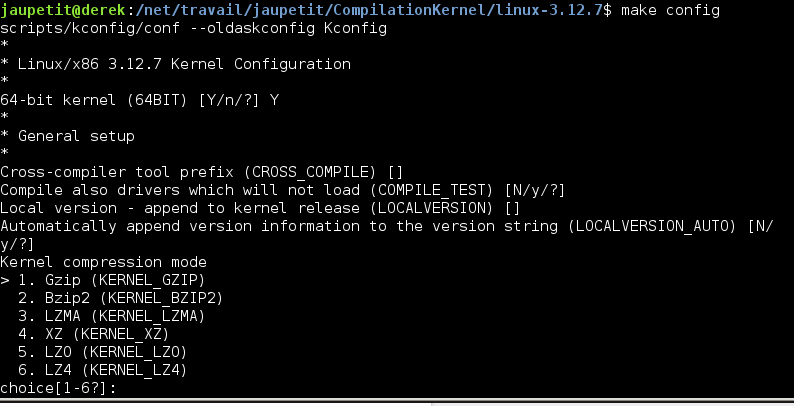
\includegraphics[scale=0.7]{illustrations/configLine.png}
            \centering
            \caption{Interface en ligne de commande}
            \label{fig:MakeConfig}
        \end{figure}
        \pagebreak
    \item[make menuconfig]      Un programme utilisant ncurse \\

        \begin{figure}[H]
            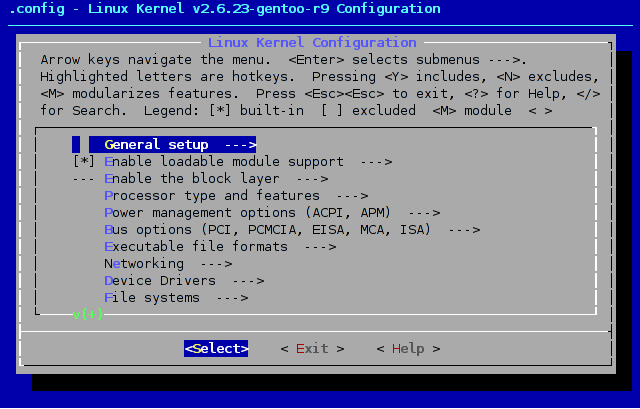
\includegraphics[scale=0.7]{illustrations/menuconfig.png}
            \centering
            \caption{Interface utilisant Ncurse}
            \label{fig:MakeMenuConfig}
        \end{figure}
\item[make xconfig]             Un programme utilisant QT \\

        \begin{figure}[H]
            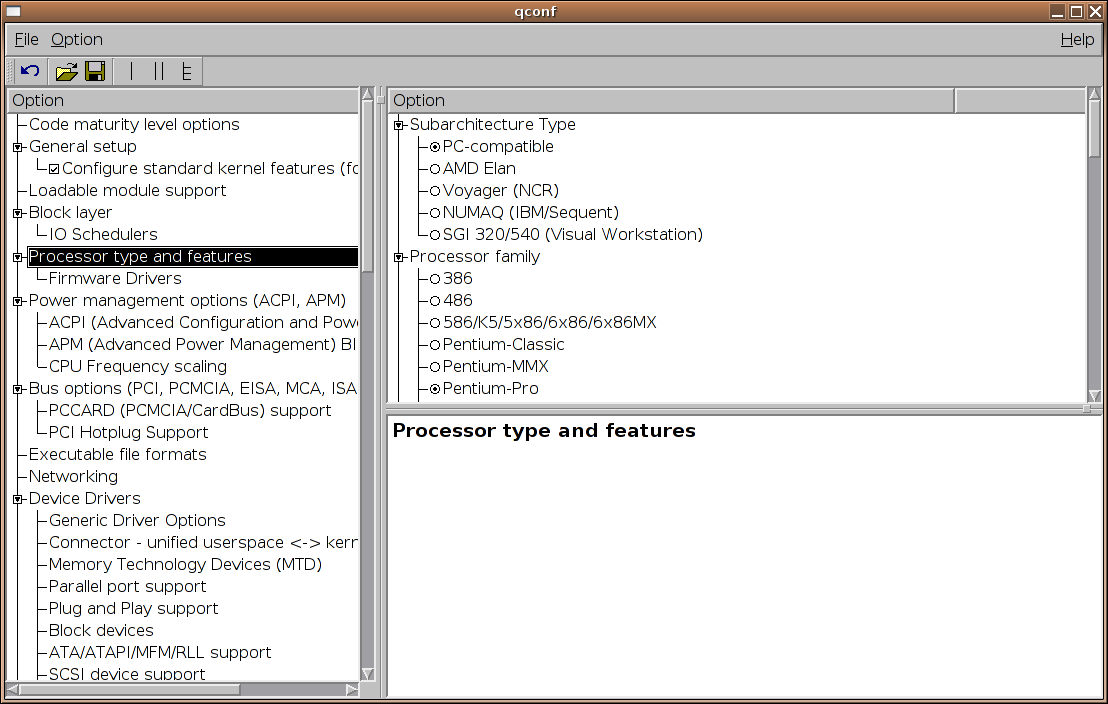
\includegraphics[scale=0.4]{illustrations/xconfig.png}
            \centering
            \caption{Interface utilisant QT}
            \label{fig:MakeXconfig}
        \end{figure}
        \pagebreak
\item[make gconfig]             Un programme utilisant GTK \\

        \begin{figure}[H]
            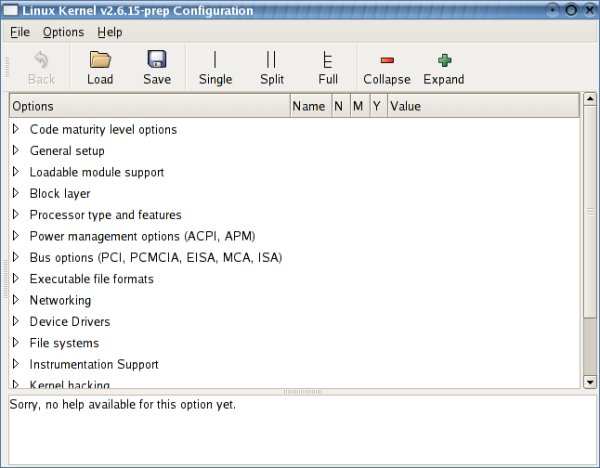
\includegraphics[scale=0.9]{illustrations/gconfig.jpg}
            \centering
            \caption{Interface utilisant GTK}
            \label{fig:MakeGconfig}
        \end{figure}
    \item[eCos], qui permet de configurer les noyaux pour le système
        d’exploitation eCos. C’est une autre source d’information
        sur laquelle se baser. \\

        \begin{figure}[H]
            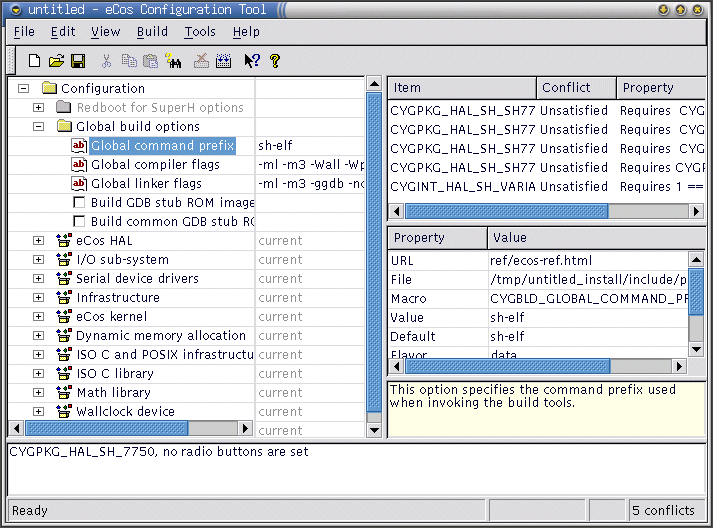
\includegraphics[scale=1.2]{illustrations/eCos_config.png}
            \centering
            \caption{Interface de configuration de noyau pour l'OS eCos}
            \label{fig:InterfaceEcos}
        \end{figure}
        \pagebreak
    \item[kcheck (kernel check)] permet également de configurer les options
        d’un noyau à compiler. \\
        Il propose deux modes : \\

    \begin{description}
        \item[Automatique :] kcheck va tenter de déterminer les options du kernel
            en fonction de la machine sur laquelle il est lancé
        \item[Manuel :] kcheck permet à l’utilisateur de modifier comme bon lui
            semble les différentes options du fichier de configuration du kernel.
    \end{description}
        \begin{figure}[H]
            
\includegraphics[scale=0.8]{illustrations/kernel_check.png}
            \centering
            \caption{Interface de configuration d'un noyau proposant la détection du matériel pour les noyaux 2.*}
            \label{fig:KernelCheck}
        \end{figure}
\end{description}

Une étude a été réalisée par Kacper Bak et Karim Ali de l’université Waterloo
afin d’améliorer la convivialité de la configuration d’un noyau Linux
\cite{Waterloo:Etude}.  \\

Celle-ci a permis de mieux cerner les besoins des utilisateurs en observant
leurs difficultés à utiliser les outils existants. Ils ont réalisé un prototype
qu’ils ont fait tester et qu’ils ont amélioré afin d’obtenir le squelette d’un
outil facilitant la configuration d’un noyau Linux. \\ \\

\begin{figure}[H]
    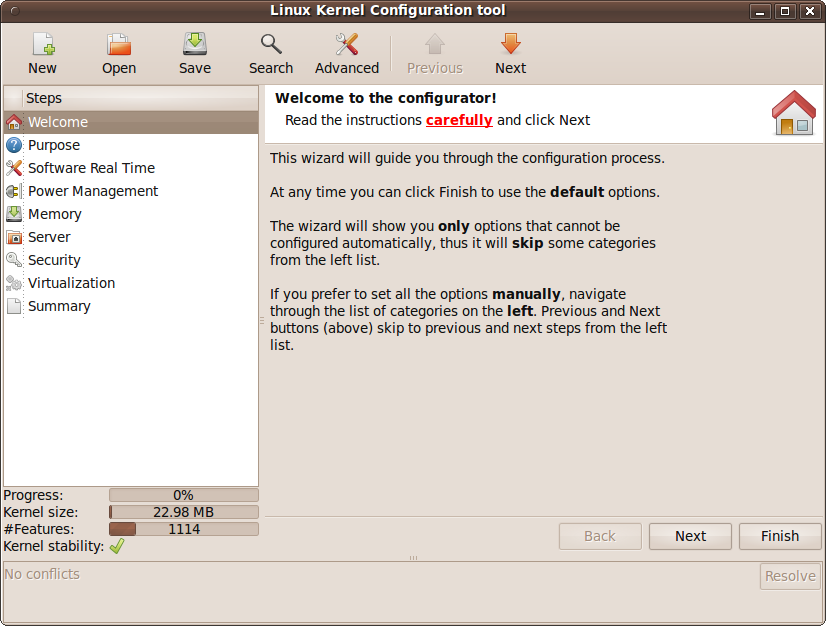
\includegraphics[scale=0.6]{illustrations/lkc_config.png}
    \centering
    \caption{Prototype de l'université de Waterloo}
    \label{fig:PrototypeWaterloo}
\end{figure}

Leur projet a donc abouti sur un prototype non fonctionnel.  L’ergonomie de
leur application sera une grande source d’inspiration pour nous grâce aux avis
qu’ils ont récoltés auprès d’utilisateurs.  \\

Les quatre premiers outils présentés ("config", "menuconfig", "xconfig" et
"gconfig") sont les plus couramment utilisés pour configurer un noyau Linux
avant sa compilation. Nous sommes arrivés à cette conclusion, car dans un
premier temps, ces outils sont présents au sein même des sources du noyau
Linux.  Et dans un second temps, en recherchant comment d'autres personnes
réalisaient cette configuration, nous avons constaté qu'ils utilisaient à
chaque fois l'un de ces outils et principalement ceux avec une interface
graphique.  \\

Pour ce qui est des deux derniers outils ("eCos", et "kCheck"), ils sont
beaucoup moins répandus, mais ils répondent à différents besoins de notre projet
dont nous allons nous inspirer :
\begin{itemize}
    \item La gestion des conflits entre les options
    \item La détection du matériel pour générer le fichier de configuration
\end{itemize}

Enfin, le dernier outil est seulement un prototype réalisé par l'université de
Waterloo, mais qui constitue notre plus importante base pour ce projet. En
effet, celui-ci ayant été réalisé après une étude des besoins des utilisateurs,
il comporte des informations précieuses pour réaliser notre PdP.  \\

\section{Difficultés de la configuration}
\label{sec:Difficultés de la configuration}


Il existe plusieurs raisons qui font que la configuration des options d’un
noyau est une tâche fastidieuse et difficile : \\

Tout d’abord, le principal problème se situe au niveau des conflits et des
dépendances entre les options. En effet, celles-ci peuvent être liées à
d’autres options ou être exclusives, c’est-à-dire que si une option est
sélectionnée, une autre peut ne plus l’être.  Le problème de certains des
outils actuels est que les options en conflit avec les options actuelles ne
sont plus visibles. Donc lorsque l’on cherche une option précise qui n’est plus
affichée et que l’on ne sait pas quelle option est en conflit avec elle, il est
très difficile de corriger cette erreur.  \\

En outre, lorsqu'une option est sélectionnée, les outils actuels désactivent
automatiquement et sans prévenir l'utilisateur celles qui sont en conflit ou
celles qui en dépendent.  \\

Enfin, il est compliqué pour un utilisateur non expert de trouver une option
précise sans la connaître parfaitement. Le nom de cette option ne représente
pas toujours très bien sa fonction, ce qui fait que la recherche des options
dans l’outil n’est pas aisée.  On constate qu’il y a une aide pour chacune des
options et il est dommage que la recherche par mots-clés ne s’effectue pas
également sur l’aide des fonctions.  \\

\section{Recherches bibliographiques}
\label{sec:Recherches bibliographiques}


Notre sujet se repose sur un projet existant. En effet, l'université de
Waterloo a réalisé une étude approfondie \cite{Waterloo:Etude} sur la facilité
d'utilisation des outils de configuration du noyau Linux. On y trouve les
résultats de leurs tests auprès de différents utilisateurs, ce qui nous permet
d'avoir des informations sur les besoins réels vis-à-vis de cet outil. L'équipe
a réalisé un prototype qui prend en compte ces modifications et celui-ci peut
être trouvé dans leur dépôt Github \cite{Waterloo:Github}.  \\

Nous avons trouvé d'autres avis d'utilisateurs au sein d'une étude
\cite{Hubaux:2012:USC:2110147.2110164}. On peut y observer les principaux
problèmes qu'ils ont rencontrés. Par exemple, on peut constater que la gestion
des conflits est une fonctionnalité qui pose généralement des difficultés.  \\

Pour mieux comprendre notre sujet, nous avons configuré et compilé un noyau
Linux que nous avons trouvé sur le site officiel \cite{Kernel}. On peut trouver
au sein du dossier téléchargé, différents outils permettant de réaliser la
configuration du noyau avant sa compilation. On y trouve "menuconfig",
"xconfig" et "gconfig" qui sont des outils graphiques plus simple d'utilisation
que l'outil en ligne de commande "config".  \\

La configuration étant difficile, nous avons trouvé sur le forum de Linux
\cite{Existant:Kernel:ForumTutoConfig} des explications très détaillées. Ce
guide reprend "pas à pas" chacune des options et les détaille une à une afin de
mieux comprendre ce qui peut être activé ou non.  \\

Une fonctionnalité qui pourrait être utile pour un utilisateur serait de
pouvoir détecter le matériel de son ordinateur (ou une partie) afin de pouvoir
générer le fichier de configuration correspondant à sa machine. Nous avons
trouvé un tutoriel \cite{Existant:Kernel:outils} traitant de la compilation du
noyau Linux et qui évoque ce point particulier.  \\

Un des problèmes évoqués par les testeurs de l'étude \cite{Waterloo:Etude} de
l'université de Waterloo, est que le système de gestion des conflits des outils
actuels n'est pas pratique, car aucune indication n'est donnée lorsqu'une
option est sélectionnée. Nous avons trouvé un outil qui effectue ce traitement
des conflits, mais pour un système d'exploitation différent : eCos
\cite{Existant:EcosConfig}. En nous en inspirant, nous pourrons éventuellement
proposer un mécanisme similaire dans notre outil de configuration.  \\

L'étude \cite{Waterloo:Etude} explique brièvement comment fonctionne
l'arborescence des modules au sein du noyau Linux. Nous avons donc décidé
d'approfondir ce point et nous avons trouvé un fichier
\cite{Existant:Kconfig:frontends} expliquant plus en détail le fonctionnement
pour l'outil "menuconfig". En reprenant le même mécanisme utilisé par les
outils officiels, nous pourrons éventuellement nous abstenir de refaire le
parsage des nombreux dossiers des sources. Nous avons également récupéré de la
documentation \cite{Existant:Kconfig:vueDensemble}
\cite{Existant:Kconfig:langage} qui contient les éléments de syntaxe qui nous
ont aidés à comprendre comment s'effectue la génération du fichier ".config".
De plus, on trouve sur le site officiel du noyau Linux des indications
\cite{Existant:Kconfig:modules} permettant de compiler un module externe au
sein du noyau. Celui-ci nous permet donc de mieux comprendre le fonctionnement
des fichiers "Kbuild".

    \section{La bibliothèque python kconfiglib}
    \label{sec:La bibliothèque python kconfiglib}
    Les fichiers Kconfig sont présents dans toute l'arborescence d'une archive linux.
    Ces fichiers regroupent toutes les options possibles pour un noyau, ainsi que
    les informations correspondantes.
    Voici un exemple extrait du fichier linux-3.13.6/arch/x86/Kconfig: \\

    \begin{verbatim}
     config X86_MPPARSE
        bool "Enable MPS table" if ACPI || SFI
        default y
        depends on X86_LOCAL_APIC
        ---help---
          For old smp systems that do not have proper acpi support. Newer systems
          (esp with 64bit cpus) with acpi support, MADT and DSDT will override it
    \end{verbatim}

    \begin{verbatim}
        un nom : X86_MPPARSE
        un type : bool
        une description / nom long : "Enable MPS table"
        des dépendances : if ACPI || SFI
        une valeur par défaut : default y
        des dépendances : depends on X86_LOCAL_APIC
        une aide : ---help---
            For old smp systems that do not have proper acpi support. Newer systems
            (esp with 64bit cpus) with acpi support, MADT and DSDT will override it
    \end{verbatim}

    Pour les besoins du projet, il nous était nécessaire de parser les fichiers
    Kconfig pour récupérer toutes les informations disponibles sur les options
    : nom, description, aide, dépendances... Avant de débuter l'implémentation
    d'un parseur, il nous a paru judicieux de vérifier si cet outil n'avait pas
    déjà été réalisé par une tierce personne.
    Nous avons trouvé sur github \cite{Existant:lib:kconfiglib} la bibliothèque
    \textit{Kconfiglib}. Cette bibliothèque est implémentée en Python, ce qui
    nous a d'ailleurs poussé vers une implémentation totale dans ce langage,
    pour être homogène avec l'API. En effet, celle-ci permet d'extraire
    facilement toutes les informations des fichier \textit{Kconfig} dont nous
    avions besoin, de générer un fichier .config, de lire un fichier .config,
    de modifier les valeurs des options quand c'est possible (s'il n'y a pas de
    conflits ou de problèmes de dépendances).
    On peux observer ci-dessous ce que nous avons utilisé dans cette API : \\

    \begin{description}
        \item[La classe Config :] Cette classe parcourt l'archive Linux à la
            recherche de ses fichiers Kconfig, afin de les parser et de générer
            en mémoire la structure qui contiendra toutes les options et leurs
            informations (nom, type, valeur, description, aide...). \\

        \item[La méthode ] \verb|Config.get_top_level_items():| Cette méthode
            retourne une liste "d'items" qui peuvent être des objets des
            classes Symbol, Menu, Choice ou Comment. Chacun d'eux hérite de la
            classe Item.  Dans notre application, nous avons eu à traiter les
            symbols, les choices et les menus.\\

            Un \textit{symbol} est une option basique, de type \textit{bool
            (oui / non)} ou \textit{tristate (oui / non / module)}. La majorité
            des options sont de la classe Symbol.  Un choice est une option de
            type string, dont la valeur est le nom d'une autre option.  Un menu
            est un item qui regroupe des options \textit{symbol et choice} en
            fonction de leurs domaines d'action (exemples : Partition Types,
            Bus options...).
        \item[La méthode ] \verb|(Symbol|\verb|Choice).get_visibility():| Cette
            fonction permet entre autre de savoir si telle ou telle option est
            modifiable. Il y a plusieurs raisons possibles pour qu'une option
            ne soit pas \textit{visible}:
            \begin{itemize}
                \item Conflit avec une ou plusieurs autres options
                \item Dépendances non satisfaites
                \item Type hexadécimal / int \newline
            \end{itemize}
        \item[La méthode ] \verb|Config.write_config():| Cette méthode est
            appelée lorsque la configuration est terminée et / ou qu'il faut
            sauvegarder le fichier. Elle génère le fichier .config à l'endroit
            voulu sur le disque.
        \item[La méthode ] \verb|Config.load_config():| Cette méthode nous sert
            à ouvrir un fichier de configuration pour le charger en mémoire,
            afin d'apporter des modifications par exemple.
    \end{description}

        \section{La bibliothèque pour le matériel}
    \label{sec:La bibliothèque pour le matériel}

    Suite à la demande concernant la génération automatique d'un fichier
    .config minimal, nous avions envisagé de détécter le matériel sur la
    machine qui executerait notre outil, et de créer une configuration associée
    en activant les options / modules correspondant. Comme pour le parsage des
    Kconfig, nous avons tout d'abord rechercher s'il n'existait pas une
    bibliothèque ou un module capable de réaliser cette tâche. Nous avons
    trouvé la bibliothèque \textit{LKDDb} \cite{Existant:lib:lkddb}. Cette
    bibliothèque permet de détecter le matériel, et, couplée à une autre
    bibliothèque \textit{AutoKernConf} \cite{Existant:lib:autoKernConf}, de
    générer un fichier de configuration minimal. \\

    LKDDb fournit un script qui permet de générer une liste de correspondance
    entre matériel et option. Voici des extraits de cette liste : \\

    \begin{verbatim}
    lkddb acpi "80860F14" :: CONFIG__UNKNOW__ :: drivers/mmc/host/sdhci-acpi.c
    lkddb acpi "80860F28" :: CONFIG_ACPI :: drivers/acpi/acpi_platform.c
    [...]
    lkddb ap 03 :: CONFIG_ZCRYPT :: drivers/s390/crypto/zcrypt_pcicc.c
    lkddb ap 04 :: CONFIG_ZCRYPT :: drivers/s390/crypto/zcrypt_pcica.c
    [...]
    lkddb ccw 1403 .. .... .. :: CONFIG_S390_VMUR :: drivers/s390/char/vmur.c
    lkddb ccw 1731 01 1732 01 :: CONFIG_QETH :: drivers/s390/net/qeth_core_main.c
    [...]
    lkddb eisa "ABP7501" :: CONFIG_SCSI CONFIG_SCSI_ADVANSYS :: drivers/scsi/advansys.c
    lkddb eisa "ADP0000" :: CONFIG_SCSI CONFIG_SCSI_AHA1740 :: drivers/scsi/aha1740.c
    \end{verbatim}

    C'est AutoKernConf qui va détecter le matériel en utilisant des outils
    Linux, tels que lspci et cat (sur des fichiers comme "/proc/cpuinfo", par
    exempe), et construire un fichier .config avec les bonnes options pour ce
    matériel. Tout ça à partir de la liste de correspondance autogénérée par
    l'API de LKDDb. \\

    Nous n'avons pas pu utiliser ce script pour plusieurs raisons :
    \begin{itemize}
        \item La dernière version des scripts n'est plus disponible. Nous avons
            seulement pu trouver une ancienne version grâce au site
            "archive.org".
        \item Les quelques tests que nous avons réalisé montrent que la liste
            d'options généré n'est pas au bon format. En effet, le script
            faisant la correspondance entre les options et le matériel attend
            un format différent.
        \item Nous avons essayé de modifier le formalisme du fichier généré
            pour faire la correspondance ensuite, mais le script récupérant le
            matériel se base sur un noyau Linux 2.* ce qui fait que la liste
            est incomplète.
    \end{itemize}

\chapter{Conception}
\label{cha:Conception}
    \section{Cahier des charges}
    \label{sec:Cahier des charges}
        \subsection{Scénarios et maquettes}
        \label{sub:Scénarios et maquettes}

\subsubsection{Scénario A: Configuration par défaut}
\label{sssub:Scénario A: Configuration par défaut}

\begin{enumerate}
    \item L'utilisateur lance l'application.
    \begin{figure}[H]
        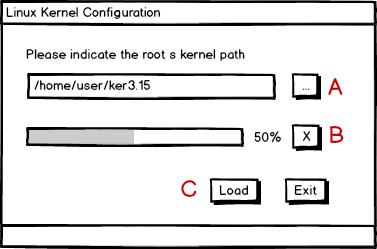
\includegraphics[scale=0.5]{illustrations/maquettes/Maquette_1_first_dialog.png}
        \centering
        \caption{Maquette 1}
        \label{fig:Maq1}
    \end{figure}
    \item L'utilisateur sélectionne le noyau qu'il souhaite configurer
            (Maquette 1 - Élément A).
    \item L'utilisateur valide le noyau qu'il a choisi (Maquette 1 - Élément C).
    \item L'application charge en mémoire les options du noyau et passe à la
            fenêtre suivante lorsque la barre de chargement est pleine (Passe à
            la Maquette 2).
    \begin{figure}[H]
        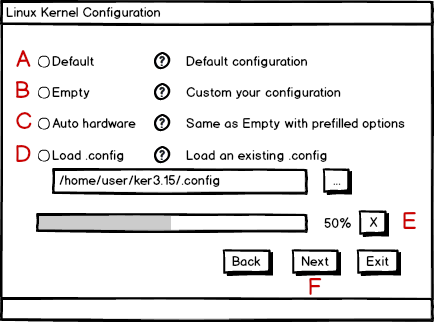
\includegraphics[scale=0.5]{illustrations/maquettes/Maquette_2_choose_dialog.png}
        \centering
        \caption{Maquette 2}
        \label{fig:Maq2}
    \end{figure}
    \item L'utilisateur sélectionne la configuration par défaut (Maquette 2 -
        Élément A).
    \item L’utilisateur clique sur Next (Maquette 2 - Élément F).
    \item L’application sélectionne les options en mémoire pour une
            configuration par défaut. Lorsque la barre de chargement est pleine,
            l’application passe à la fenêtre suivante.
    \begin{figure}[H]
        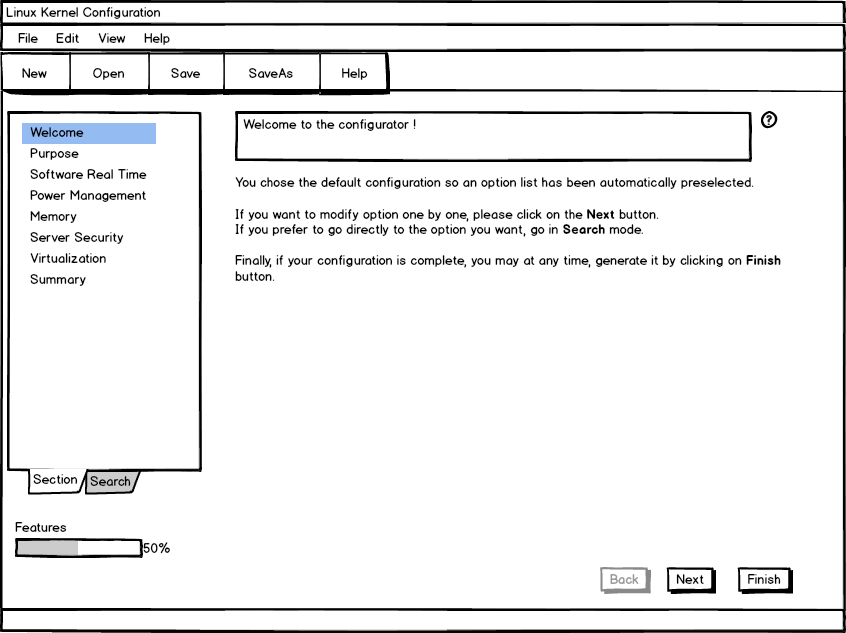
\includegraphics[scale=0.5]{illustrations/maquettes/Maquette_3_MainWindowStart.png}
        \centering
        \caption{Maquette 3}
        \label{fig:Maq3}
    \end{figure}
    \item L’utilisateur valide les options pré-sélectionnées en cliquant sur
        Finish (Maquette 3).
    \item L’application génère le fichier “.config”.
    \item L’utilisateur quitte l’application.
\end{enumerate}

\subsubsection{Scénario B: Configuration avancée, modifications, conflits}
\label{sssub:Scénario B: Configuration avancée, modifications, conflits}

\begin{enumerate}
    \item Reprendre le scénario A jusqu’à l’étape 4.
    \item L’utilisateur sélectionne la configuration vierge / empty  (Maquette
        2 - Élément B).
    \item L’utilisateur clique sur Next (Maquette 2 - Élément F).
    \item L’application passe à la fenêtre suivante (Passe à la Maquette 3).
    \item L’utilisateur clique sur “next” et l’application passe sur la
        première option (Passe à la Maquette 4).
    \begin{figure}[H]
        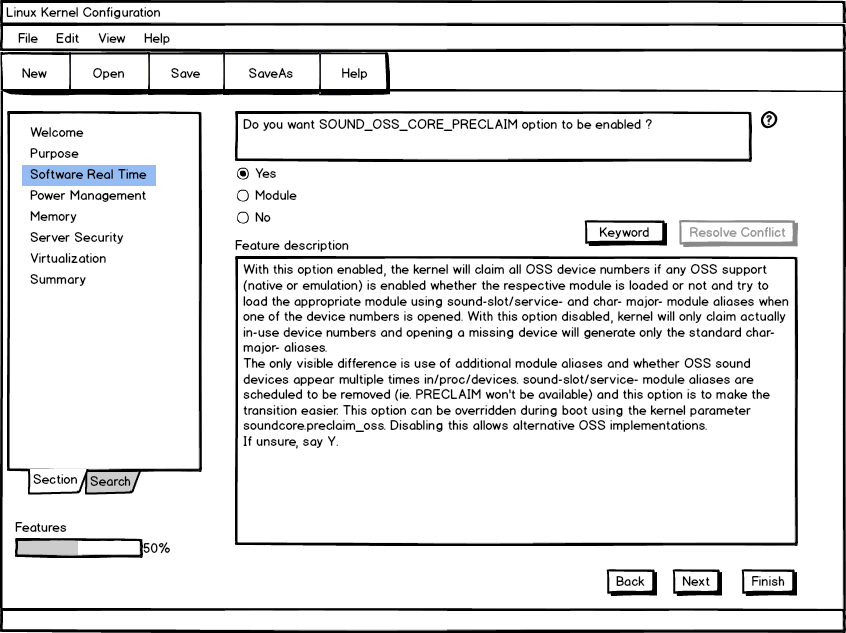
\includegraphics[scale=0.5]{illustrations/maquettes/Maquette_4_MainWindowSection.png}
        \centering
        \caption{Maquette 4}
        \label{fig:Maq4}
    \end{figure}
    \item L’utilisateur clique sur “next” (Maquette 4), ce qui valide le choix
        précédent (l’option est à “yes” par défaut) et passe à l’option suivante.
    \item L’application précise qu’il y a un conflit (l’option est à “yes” par
        défaut) et n’autorise pas l'utilisateur à cliquer sur “next” (Maquette 5).
    \begin{figure}[H]
        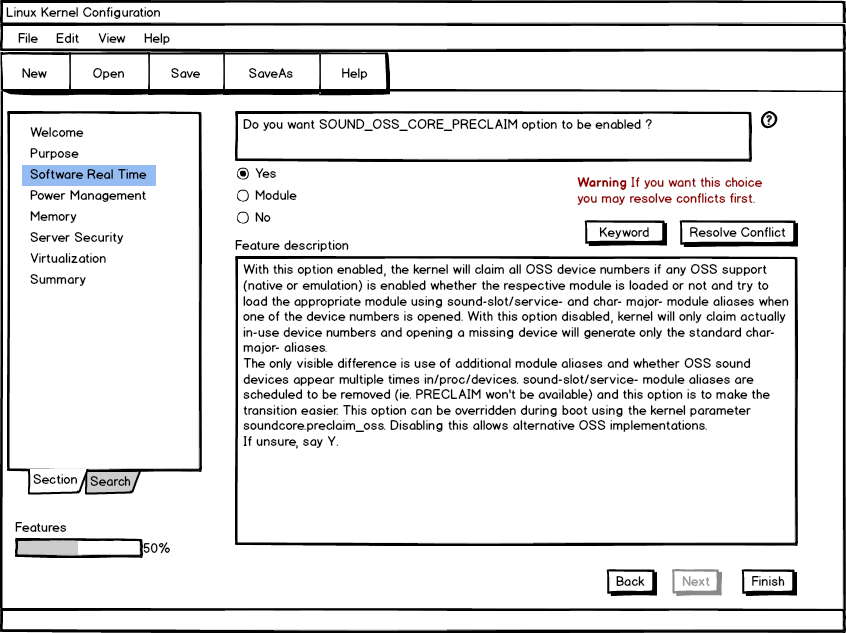
\includegraphics[scale=0.5]{illustrations/maquettes/Maquette_5_MainWindowSectionConflict.png}
        \centering
        \caption{Maquette 5}
        \label{fig:Maq5}
    \end{figure}
    \item L’utilisateur clique sur “resolve conflict” (Maquette 5).
    \item L’application ouvre une fenêtre de résolution des conflits (Maquette
        6) et affiche toutes les options en conflit.
    \begin{figure}[H]
        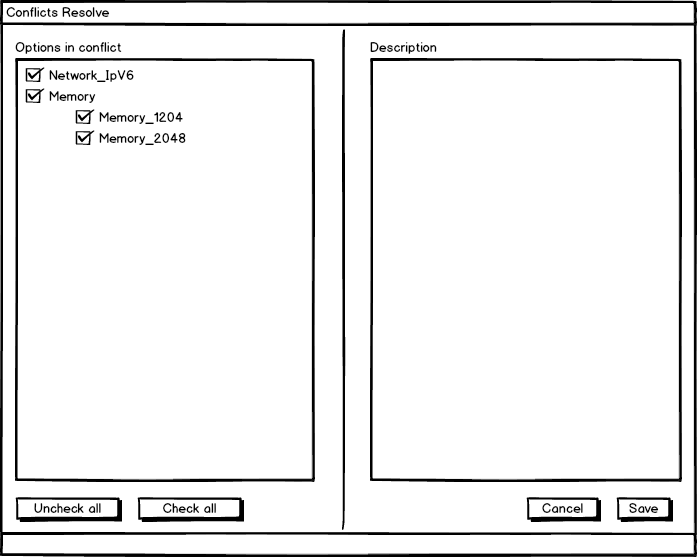
\includegraphics[scale=0.5]{illustrations/maquettes/Maquette_6_resolve_dialog.png}
        \centering
        \caption{Maquette 6}
        \label{fig:Maq6}
    \end{figure}
    \item L’utilisateur clique sur “uncheck all” et valide son choix en cliquant
        sur save (Maquette 6).
    \item L’application applique les changements apportés par l’utilisateur et
        revient à la fenêtre principale (Maquette 4).
    \item L’utilisateur peut dorénavant sélectionner l’option qu’il voulait et
        il clique donc sur “next” (Maquette 4).
    \item L’utilisateur valide les options sélectionnées en cliquant sur Finish
        (Maquette 4).
    \item L’application génère le fichier “.config”.
    \item L’utilisateur quitte l’application.
\end{enumerate}

\subsubsection{Scénario C: Configuration par détection du matériel, recherche d'options}
\label{sssub:Scénario C: Configuration par détection du matériel, recherche d'options}

\begin{enumerate}
    \item Reprendre le scénario A jusqu’à l’étape 4.
    \item L’utilisateur sélectionne la configuration détection du matériel /
        auto hardware (Maquette 2 - Élément C).
    \item L’utilisateur clique sur Next (Maquette 2 - Élément F).
    \item L’application sélectionne les options qui coïncident avec le matériel
        de l’utilisateur. Lorsque la barre de chargement est pleine,
        l’application passe à la fenêtre suivante (Passe à la Maquette 3).
    \item L’utilisateur clique sur Search (Passe à la Maquette 7).
    \begin{figure}[H]
        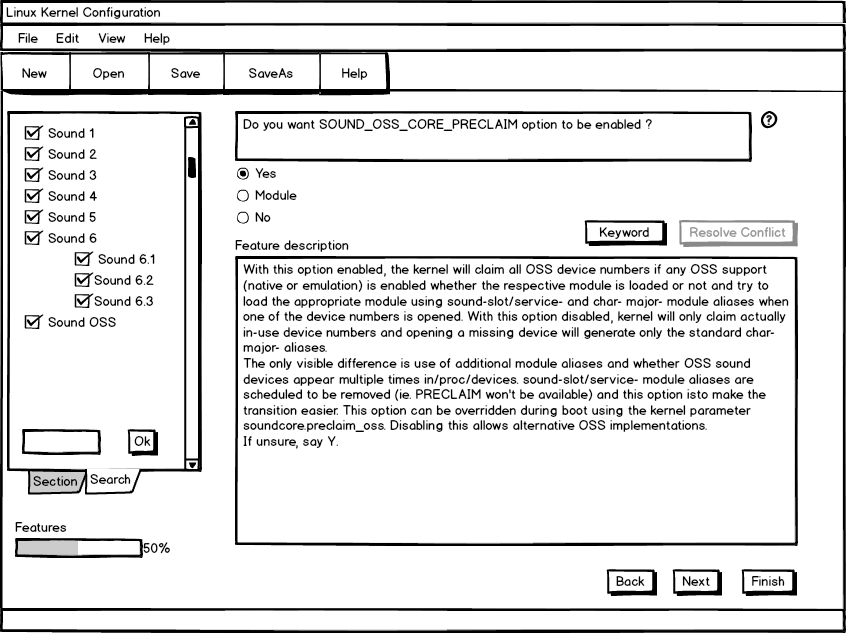
\includegraphics[scale=0.5]{illustrations/maquettes/Maquette_7_MainWindowSearch.png}
        \centering
        \caption{Maquette 7}
        \label{fig:Maq7}
    \end{figure}
    \item L’application affiche une zone de saisie.
    \item L’utilisateur saisit un mot clé pour trouver une option.
    \item L’application affiche les options relatives à ce mot-clé (Maquette 8).
    \begin{figure}[H]
        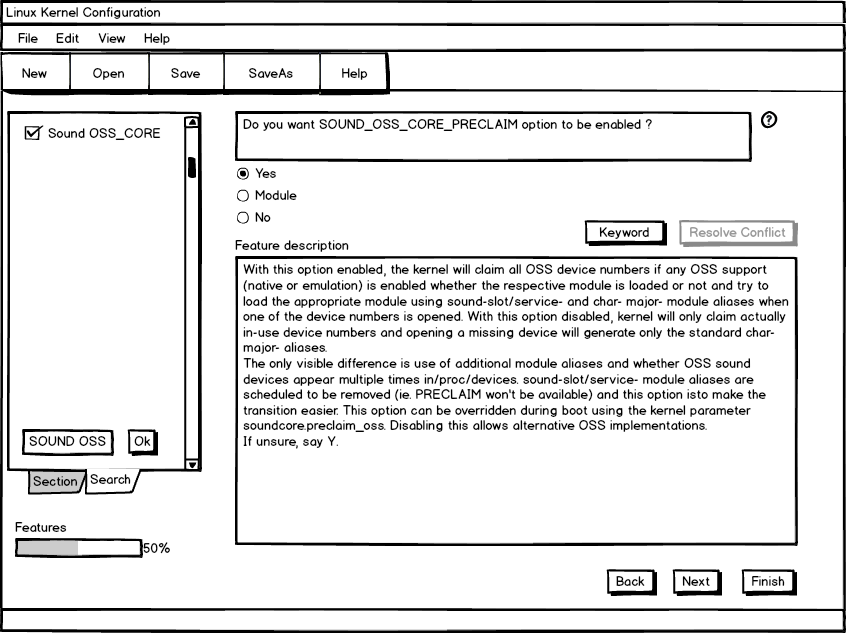
\includegraphics[scale=0.5]{illustrations/maquettes/Maquette_8_MainWindowSearchResult.png}
        \centering
        \caption{Maquette 8}
        \label{fig:Maq8}
    \end{figure}
    \item L’utilisateur peut sélectionner l’option qu’il voulait.
    \item L’utilisateur valide les options sélectionnées en cliquant sur Finish
        (Maquette 8).
    \item L’application génère le fichier “.config”.
    \item L’utilisateur quitte l’application.
\end{enumerate}

\subsubsection{Scénario D: Configuration par chargement de fichier de configuration, ajout de mots-clés}
\label{sssub:Scénario D: Configuration par chargement de fichier de configuration, ajout de mots-clés}


\begin{enumerate}
    \item Reprendre le scénario A jusqu’à l’étape 4.
    \item L’utilisateur sélectionne la configuration Load .config (Maquette 2 -
        Élément D).
    \item L’application sélectionne les options présentent dans le fichier
        précédemment chargé.
    \item L’utilisateur clique sur Next (Maquette 2 - Élément F).
    \item L’application sélectionne les options présentent dans le fichier
        précédemment chargé. Lorsque la barre de chargement est pleine,
        l’application passe à la fenêtre suivante (Passe à la Maquette 3).
    \item L’utilisateur sélectionne une option et clique sur Keyword (Passe à
        la Maquette 9).
    \begin{figure}[H]
        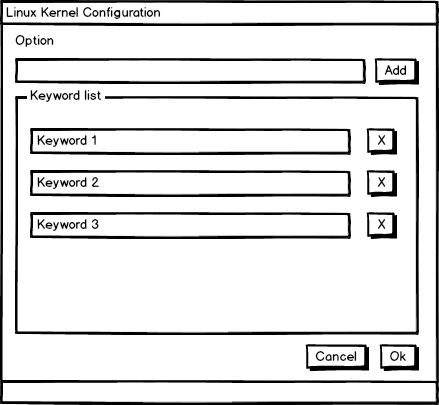
\includegraphics[scale=0.5]{illustrations/maquettes/Maquette_9_keyword_dialog.png}
        \centering
        \caption{Maquette 9}
        \label{fig:Maq9}
    \end{figure}
    \item L’utilisateur saisit le nom d’un mot-clé et valide l’ajout.
    \item L’utilisateur valide les options sélectionnées en cliquant sur Finish.
    \item L’application génère le fichier “.config”.
    \item L’utilisateur quitte l’application.
\end{enumerate}


        \subsection{Diagramme des cas d'utilisations}
        \label{sub:Diagramme des cas d'utilisations}

\begin{figure}[H]
    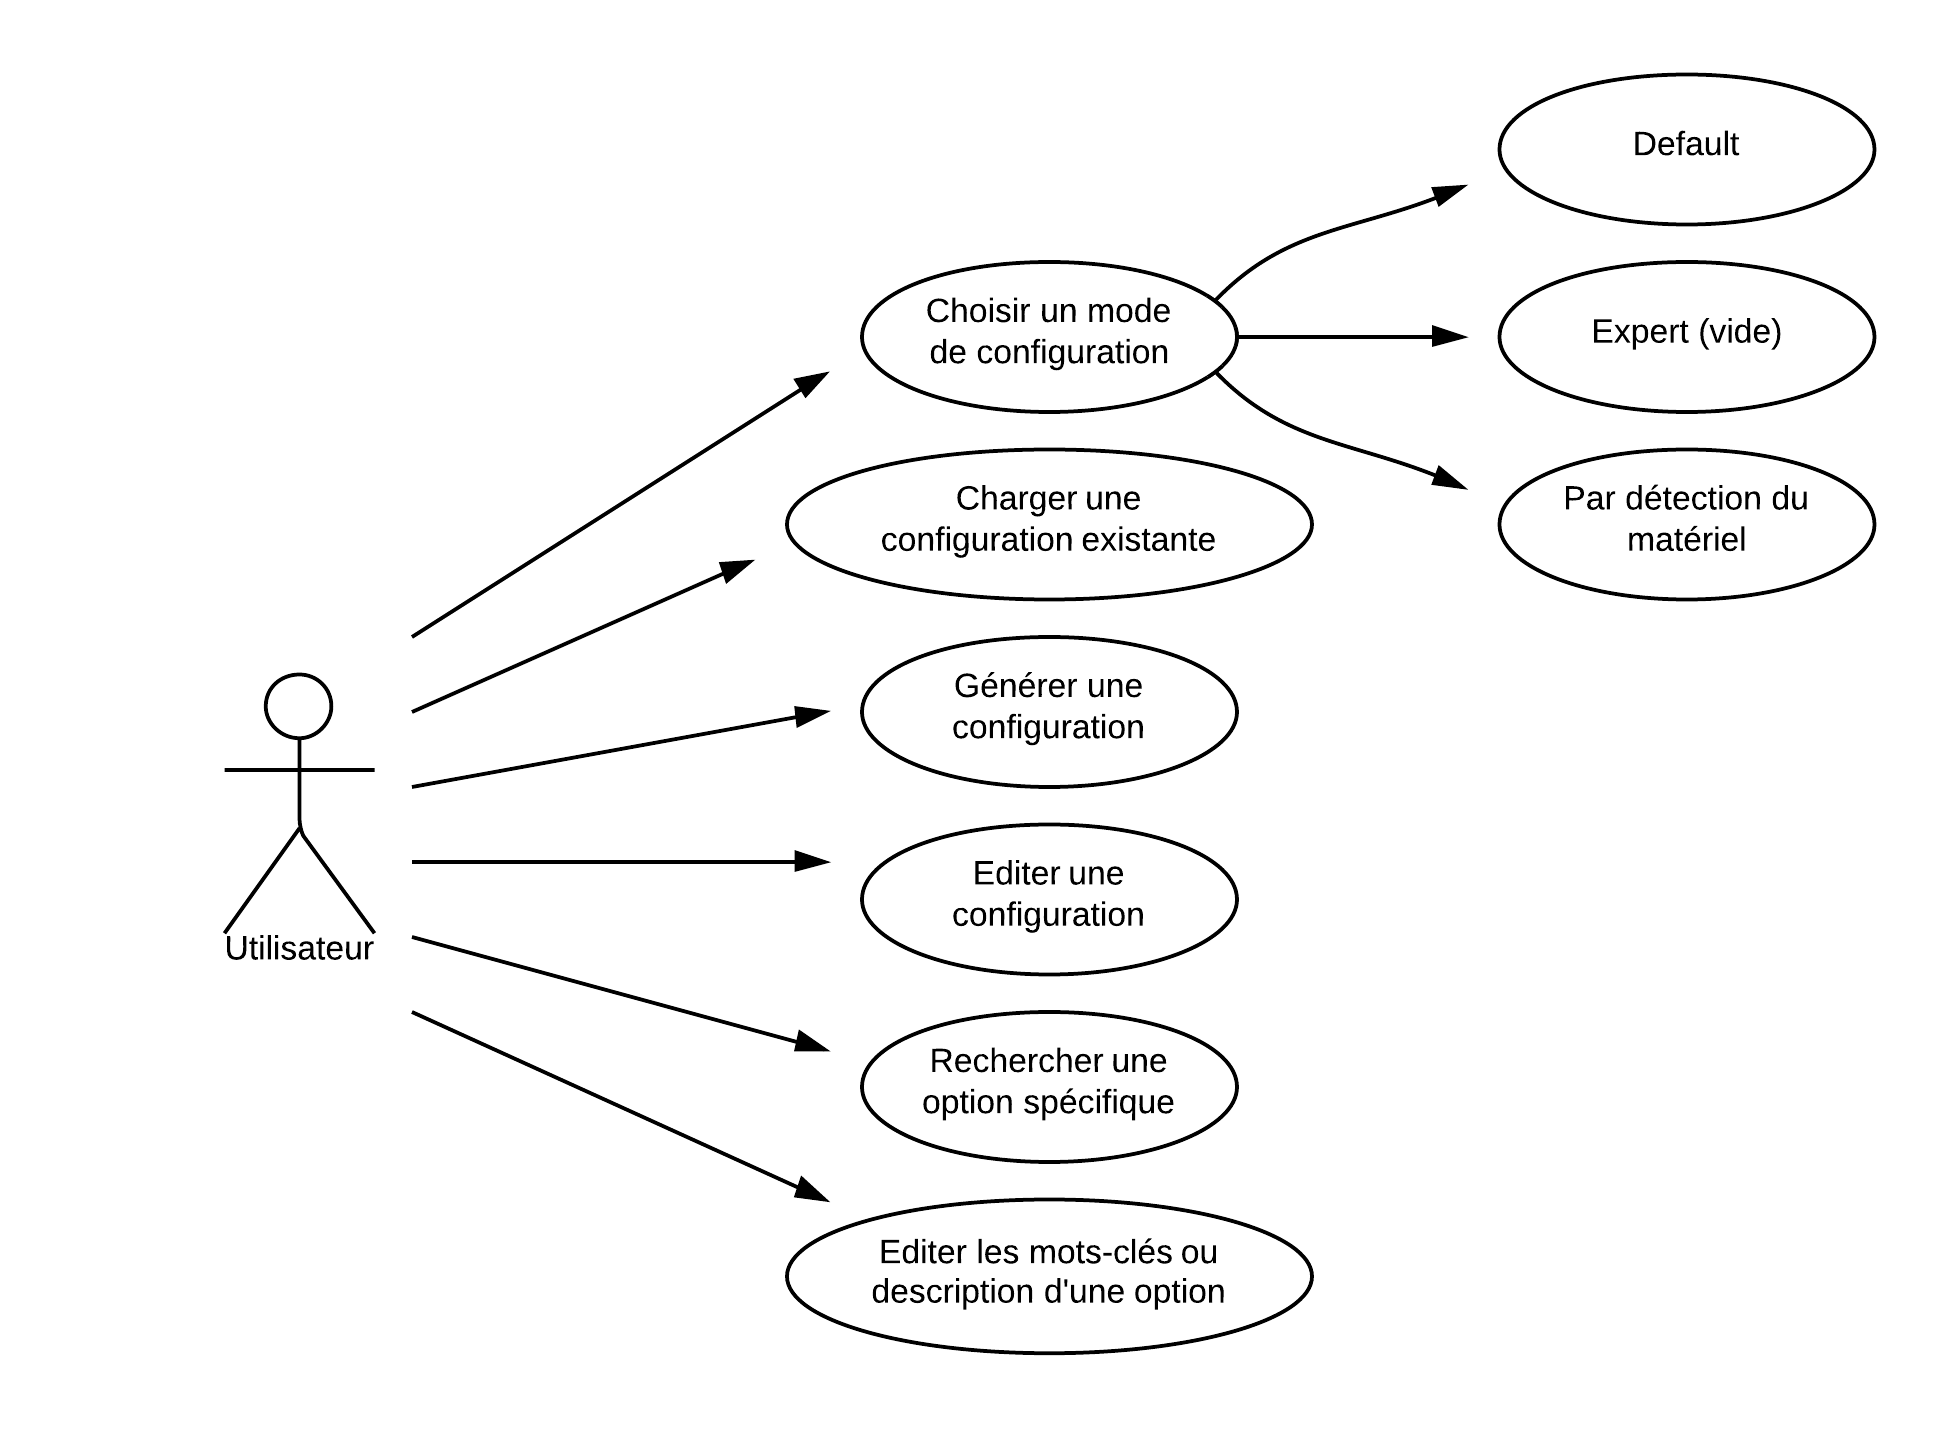
\includegraphics[scale=0.25]{illustrations/diagramme_cas_utilisation.png}
    \centering
    \caption{Diagramme des cas d'utilisation}
    \label{fig:DCU}
\end{figure}

        \subsection{Besoins fonctionnels et tests prévus}
        \label{sub:Besoins fonctionnels et tests prévus}

\subsubsection{Détection du matériel}
\label{ssub:Détection du matériel}
\paragraph{Besoin}
\label{sssbus:Besoin}

Il faut qu’un utilisateur puisse détecter son matériel afin de pouvoir
avoir une liste d’options sélectionnées plus précise/adaptée qu’une
configuration par défaut. Un utilisateur désirant un noyau minimal est
confronté aux soucis qui sont de trouver la correspondance entre son matériel et
les options proposées.
\\

Il existe des outils Linux permettant de récupérer la liste du matériel associé
aux bus PCI et USB de la machine hôte.  N’ayant pas trouvé d’outil Linux
permettant de récupérer directement le ou les modules noyau utilisés sur une
entrée, l’étude du contenu des répertoires “/dev /sys” et “/proc” sera
nécessaire afin d’acquérir de plus amples informations.
\\

Afin de rendre la correspondance des modules du noyau Linux au matériel plus
pertinente et fiable, l’idée serait de récupérer des logs d’exécution du scan
du matériel afin de peupler de manière volontaire une base de données
communautaire.

\paragraph{Test}
\label{sssbus:Test}

Si l’utilisateur précise qu’il réalise une configuration pour la machine
courante, l’application devra l’alerter quand celui-ci cherchera à activer une
option incompatible avec son matériel. Par exemple, si sa machine a un
processeur 32-bits et que l’utilisateur sélectionne l’option pour un processeur
64-bits, l’application devra l’avertir que la configuration ne sera pas adaptée
à sa machine. Des tests similaires pourront être proposés pour de nombreuses
options liées au matériel.


\subsubsection{Gestion des conflits}
\label{sec:Gestion des conflits}
\paragraph{Besoin}
\label{sub:Besoin}

L’application doit pouvoir “gérer les conflits et les dépendances” entre les
options de configuration. Grâce au fichier kconfig, l’application pourra, pour
chaque option de configuration, connaître ses dépendances et les options avec
lesquelles elle rentre en conflit. De ce fait, chaque fois que l’utilisateur
sélectionne ou désélectionne une option de configuration, des tests sont
effectués par l'application pour savoir si cette option entre en conflit avec
une autre (si elle est cochée) ou génère une erreur de dépendance (si elle est
décochée).

\paragraph{Test}
\label{sub:Test}

La sélection d’une option doit signaler à l’utilisateur l’éventuelle présence
d’un conflit. Il doit également lui être proposé de pouvoir le résoudre. Or,
trouver une solution est un problème NP-complet. En effet, à chaque nouvelle
option il faut vérifier les dépendances de toutes les options précédemment
cochées. Il est possible qu’une option précédente exclût la nouvelle option.
Toutes les options du fichier de configuration en cours d’édition doivent être
vérifiées, ce qui est impossible en un temps polynomial.
\\

Il faudrait vérifier que les conflits présents dans les fichiers Kconfig du
noyau soient bien affichés dans notre outil.


\subsubsection{Recherche}
\label{sec:Recherche}
\paragraph{Besoin}
\label{sub:Besoin}

L’utilisateur doit pouvoir effectuer une recherche sur le nom, la description
et les mots-clés relatifs à une option lors de la configuration du noyau. La
fonction de recherche ne posera pas de véritable problème technique.
L’utilisateur pourra faire défiler les lignes contenant les occurrences du
terme recherché.

\paragraph{Test}
\label{sub:Test}

Vérifier que la fonction de recherche retourne bien les résultats attendus. Par
exemple, nous pourrons ouvrir un des outils existants (xconfig, gconfig) et
réaliser une recherche. On effectuera la même recherche sur notre outil et on
pourra vérifier si les résultats sont similaires (ce test ne sera valable que
pour les titres des options).


\subsubsection{Génération et chargement du fichier .config}
\label{sec:Génération et chargement du fichier .config}
\paragraph{Besoin}
\label{sub:Besoin}

L’utilisateur doit pouvoir sauvegarder où il le souhaite le fichier de
configuration généré par l’application. Un message avertira l’utilisateur de la
présence de conflits ou d’erreurs de dépendance avant que la génération ne soit
faite.
\\

La reprise d’un fichier .config doit permettre à un utilisateur de charger une
configuration existante. Le chargement d’un fichier .config corrompu provoquera
une erreur, et les options inconnues (s’il y en a) seront simplement ignorées.
Cela impliquera le déclenchement du mécanisme de résolution des conflits.

\paragraph{Tests}
\label{sub:Tests}

Vérifier que le fichier de configuration (.config) soit compatible avec
l’application lors de son chargement. Ce dernier doit respecter le format
d’origine, afin que nous puissions récupérer les informations qui nous sont
utiles.
\\

Vérifier que le fichier de configuration que nous générons via notre outil
peut être chargé (toujours via notre outil) et qu’il contienne les mêmes
données. Pour réaliser ce test, on générera à nouveau un fichier de
configuration et on pourra vérifier après ces trois étapes (génération >
chargement > génération) si les informations sont restées les mêmes. Cela
montrera que la génération et le chargement fonctionnent correctement.


\subsubsection{Mots-clés et description d'une option}
\label{sec:Mots-clés et description d'une option}

Un utilisateur doit pouvoir sélectionner une option et y ajouter un mot-clé.
Par exemple, il peut spécifier qu’une option possède le mot-clé “Network”. Il
pourra également supprimer et modifier les mots-clés existants. De la même
façon, l’utilisateur pourra éditer la description d’une option.

\subsubsection{Plateforme de partage communautaire}
\label{sec:Plateforme de partage communautaire}

S’il le souhaite, l’utilisateur peut envoyer sur la plateforme de partage, la
correspondance entre le matériel et le module capable de le faire fonctionner,
enrichissant ainsi la base de données de la plateforme.  De la même façon, lors
de la détection du matériel, l’application pourra trouver les modules à activer
(dans le fichier .config) grâce à cette plateforme. Celle-ci servira également
à stocker les “descriptions” et les “mots-clés” des options.

        \subsection{Besoins non fonctionnels}
        \label{sub:Besoins non fonctionnels}
\subsubsection{Facilité d'utilisation}
\label{sec:Facilité d'utilisation}

Notre projet consiste à améliorer l’utilisation des fonctionnalités de base des
outils existants, en les rendant plus accessibles. On a pu constater que le
système de recherche des options n’est pas simple à prendre en main et que la
gestion des conflits pouvait être améliorée.
\\

Nous avons décidé d’améliorer la recherche en scrutant au sein des descriptions
des options en plus de leurs noms. De plus, nous affichons les options pouvant
créer des conflits, ainsi que des informations sur leur provenance.

\subsubsection{Profil des utilisateurs}
\label{sec:Profil des utilisateurs}

Actuellement, les outils de configuration d’un noyau Linux sont “réservés” aux
personnes averties. Il faut donc que les fonctionnalités recherchées soient
présentes. Ces améliorations permettront de toucher un plus large public, de
débutant à expert.

\subsubsection{Portabilité}
\label{sec:Portabilité}

Il y a deux aspects liés à la portabilité. Dans un premier temps, il est
possible que l’environnement dans lequel l’application sera exécutée ne possède
pas de serveur X (interface graphique). Par conséquent, une solution
privilégiant une interface console (comme Ncurse) serait donc intéressante
puisqu’elle conviendrait à la fois à l’utilisation de l’application sur un
serveur et sur un ordinateur personnel (ou même sur tout type de support
supportant un noyau Linux). Cependant, l’application se voulant être tout
public, une interface lancée depuis la console pourrait se montrer un peu
austère pour un utilisateur habitué à une interface graphique plus
“traditionnelle”.  Dans un second temps, l’application pourra être
fonctionnelle sur un système d’exploitation Windows.

\subsubsection{Contraintes légales}
\label{sec:Contraintes légales}

Cet outil étant, open source, nous avons choisi d’utiliser la licence GPLv3.
Cela permettra la reprise éventuelle de ce projet dans l’avenir.

\subsubsection{Interface web}
\label{sec:Interface web}

L’utilisateur devrait pouvoir réaliser la détection de son matériel à partir
d’une interface web (comme le site : ma-config.com).

        \subsection{Priorité des besoins}
        \label{sub:Priorité des besoins}

\begin{tabular}{|c|c|}
    \hline
    Besoin & Priorité \\
    \hline
    \hline
    Génération du fichier .config & Haute \\
    \hline
    Gestion des conflits & Haute \\
    \hline
    Chargement d'un fichier .config & Haute \\
    \hline
    Utilisation de l'application sur un bureau & Haute \\
    \hline
    Recherche & Haute \\
    \hline
    Mots-clés et description d'une option & Moyenne \\
    \hline
    Plateforme de partage communautaire & Moyenne \\
    \hline
    Détection du matériel & Moyenne \\
    \hline
    Peuplement de la base pour la détection de matériel & Faible \\
    \hline
    Utilisation de l'application sur un serveur & Faible \\
    \hline
\end{tabular}

    
    \section{Recherches effectuées}
    \label{sec:Recherches effectuées}
        \subsection{Problème NP-Complet}
        \label{sub:Problème NP-Complet}

Au début, nous avions la volonté de permettre à l'utilisateur de pouvoir
résoudre automatiquement un conflit. Cela nous semblait faisable, mais 
nous avons découvert plus tard que pour résoudre les conflits d'une option
il fallait résoudre tous les conflits des options impliquées dans le premier
conflit et ainsi de suite jusqu'à ce qu'il n'y ait plus de conflit, mais nous 
nous sommes rendu compte que l'arbre de dépendance de certaine option pouvait être 
très profond. Nous avons pris connaissance plus tard que le problème auquel on 
était confronté était qualifié de np-complet et qu'il allait être très difficile
de tenter de le résoudre. 

%TODO
%(a = true, b = true, c = false, d = false, e = true)
%
%(a ^ b ^ c ) v ( ]c ^ d ^ e ) -> calcul en temps polynomial

%                        On peut remplacer directement et tester

%(a = true, b = e && !d , c = True, d = a, e = False)


\begin{figure}[H]
    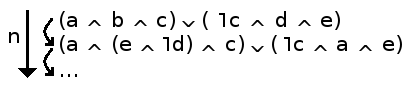
\includegraphics[scale=1]{./illustrations/np_complet.png}
    \centering
    \caption{Représentation du problème np-complet}
    \label{fig:np-complet}
\end{figure}

Nous avons décidé d'allouer une partie de notre temps de travail à la recherche
d'une façon de résoudre un problème np-complet. Lorsque nous avons compris 
qu'une solution serait tres difficle à trouver, surtout avant l'échéance, nous
avons décidé d'abandonner les recherches et de tenter une approche différente
(détaillée ci-dessous).


        \subsubsection{Détection d'une partie des conflits (getlucky)}
            \label{sub:Problème NP-Complet (getlucky)}

Résoudre tous les conflits présents sur toutes les options prendrait trop de temps.
Nous avons donc tenté une autre approche, où nous tentons de résoudre le plus 
de conflits avec une certaine limite de profondeur. Si les conflits ne sont pas
résolus lorsque nous atteignons cette limite, l'application abandonne la 
résolution et indique à l'utilisateur qu'elle n'a pas réussi à résoudre les 
conflits et invite donc l'utilisateur à le faire lui-même.\\

Exemple :\\
\begin{lstlisting}
Option Z = OptionA && !OptionB
Option A = OptionC && OptionD
Option B = OptionK
Option C = OptionW && OptionX && OptionY
Option D = OptionL && !OptionJ
\end{lstlisting}

On part d'un état initial où toutes les options sont à la valeur :
\textit{Non}.  Si l'utilisateur cherche à activer l'option Z l'option A doit
être à la valeur : \textit{Oui}. La résolution des conflits va donc tenter de
la placer à \textit{oui}, mais il va échouer, parce que les conditions de A ne sont elles
même pas respectées, c'est pourquoi, il va tenter de résoudre les conflits de A, mais
pour cela il doit mettre les valeurs de C et D à oui à condition qu'il n'y ait
pas de conflit, et ainsi de suite.  L'application descend donc récursivement dans chacune
des options pour tenter de résoudre les conflits et donner aux options la bonne
valeur. Mais dans le cas de la détection partielle des conflits, il ne va pas
descendre indéfiniment. Dans l'exemple ci-dessus, nous pouvons imaginer que
s'il ne parvient pas à résoudre les conflits de C et D, il abandonne et
indique à l'utilisateur que la résolution de conflit a échoué (puisque la
résolution de conflit automatique n'a pas réussi à mettre la valeur de A à oui
et donc à mettre la valeur de Z à oui).\\
\\

Cet algorithme peut sembler assez simple à implémenter, mais il reste encore
à trouver le moyen de déterminer les valeurs des options pour lequelles la
dépendance est validée. Pour cela nous avons trouvé deux altérnatives, la
resolution par bruteforce et la résolution par dpll.

% === TODO ===

            \subsubsection{Résoudre les équations de conflits par brute-force}
            \label{sub:Résoudre les équations de conflits par brute-force}

%TODO Expliquer brute-force
Pour trouver le résultat d'une équation de conflit, nous avons d'abord tenté
l'approche par brute-force où le but était de donner à toutes les variables
toutes les valeurs possibles et de sélectionner les combinaisons d'options qui
valident l'équation.
\\

Exemple d'équation :
\[[OptionC || (OptionA \&\& !OptionB)]\]

Pour trouver les valeurs que les options A, B et C doivent prendre, on fait
varier leurs valeurs à l'aide d'une table de vérité.  \\
\begin{tabular}{|c|c|c||c|}
    \hline
    OptionA & OptionB & OptionC & Résultat\\
    \hline
    \hline
    0 & 0 & 0 & 0\\
    \hline
    0 & 0 & 1 & 0\\
    \hline
    0 & 1 & 0 & 1\\
    \hline
    0 & 1 & 1 & 0\\
    \hline
    1 & 0 & 0 & 1\\
    \hline
    1 & 0 & 1 & 1\\
    \hline
    1 & 1 & 0 & 1\\
    \hline
    1 & 1 & 1 & 1\\
    \hline
\end{tabular}
\newline
\newline

On déduit de ce tableau que les combinaisons suivantes fonctionnent:
\begin{itemize}
    \item A = Oui et B = ?   et C = ?   \\
    \item A = ?   et B = Oui et C = Non \\
\end{itemize}

Si cette approche est assez simple à mettre en place et à comprendre, elle
n'est pas vraiment optimisée. En effet le nombre d'options dans une condition
peut être parfois très élevé, par exemple \verb|IRQ Domain| contient pas
moins de 40 options.\\
Pour trouver tous les résultats d'une telle équation il faut une table
de vérité de $1.0995116e+12$ lignes ($2^{40}$). Dans cette situation même
un ordinateur puissant mettra beaucoup de temps à créer cette table.
\\
Voici le temps pour la création d'une table de vérité sur une machine du cremi : 

\begin{tabular}{|c|c|}
    \hline
    Nombre options & temps\\
    \hline
    \hline
    4 & 0.018s\\
    \hline
    8 & 0.020s\\
    \hline
    16 & 0.726s\\
    \hline
    24 & 5m29.844s\\
    \hline
\end{tabular}
\newline
\newline

L'approche par brute-force n'est donc définitivement pas la bonne, même si les
conflits impliquant plus de 20 options ne sont pas nombreux. Peu de temps après,
nous avons tenter de résoudre ce problème avec le DPLL.\\

%Faudra un peu plus dire des trucs ici. === TODO ===

            \subsubsection{Résoudre les équations de conflits par DPLL}
            \label{sub:Résoudre les équations de conflits par DPLL}

        \subsection{Problème de détection du matériel}
        \label{sub:Problème de détection du matériel}

    \section{Évolutions}
    \label{sec:Évolutions}
        \subsection{Évolution des besoins}
        \label{sec:Évolution des besoins}

Durant la phase de conception de notre projet, nous nous sommes confrontés à 
deux difficultés qui ont fait évoluer nos besoins. En effet, nos recherches 
non pas permis de pouvoir résoudre les conflits automatiquement ni de générer 
une configuration par défaut en fonction du matériel de l'utilisateur, comme
cela a été évoqué précédemment. 
\\

L'objectif de résolution automatique des conflits a été modifié afin de 
simplement aider l'utilisateur à trouver les conflits d'une option. Il se 
chargera de modifier les valeurs des options par lui-même.
\\

En ce qui concerne le besoin de détecter le matériel d'un utilisateur, celui-ci 
s'est transformé pour devenir une base de données communautaire. Celle-ci est 
modifiable à l'aide d'un site web. Il est possible d'ajouter des relations 
entre des options et des modules, et entre des modules et du matériel. Les 
modules représentent la partie Driver. Un second besoin était de pouvoir 
ajouter des Tags aux options afin de pouvoir les regrouper afin d'affiner la 
recherche. Ce besoin a également été ajouté sur cette base communautaire.

        \subsection{Évolution de l'interface}
        \label{sub:Évolution de l'interface}

En parallèle de l'évolution des besoins, l'ergonomie de l'interface a changé 
afin d'améliorer l'utilisation de l'application et afin de correspondre aux 
fonctionnalités attendues.

\begin{enumerate}

    \item Évolution de l'interface de configuration de l'application
    \\

    L'interface de configuration permet à l'utilisateur de choisir le noyau 
    et l'architecture qu'il désire. Il peut également charger un fichier de 
    configuration existant.

    \begin{figure}[H]
        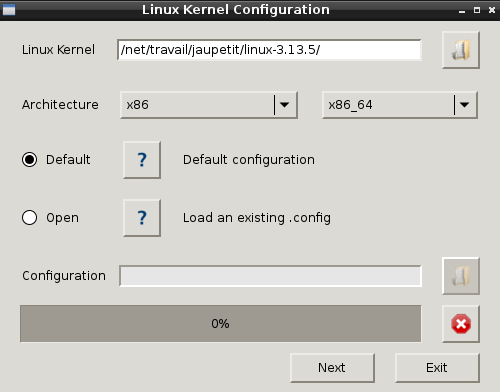
\includegraphics[scale=0.7]{./illustrations/screen_configuration_interface.png}
        \centering
        \caption{Évolution de l'interface de configuration de l'application}
        \label{fig:Evo_config}
    \end{figure}

    L'utilisateur n'a plus que deux choix contre quatre auparavant. En effet, 
    il ne peut plus détecter son matériel automatiquement comme cela était 
    le cas sur les maquettes. Il ne peut plus créer une configuration vierge, 
    car certaines options sont nécessaires pour ne pas créer de conflits.
    \\

    \pagebreak  
    \item Évolution de l'interface d'affichage des options
    \\

    L'interface de modification des options autorise l'utilisateur à naviguer 
    entre les options avec différents menus. Il peut modifier leurs valeurs 
    s'il n'y a pas de conflit et générer un fichier de configuration lorsqu'il 
    a terminé.

    \begin{figure}[H]
        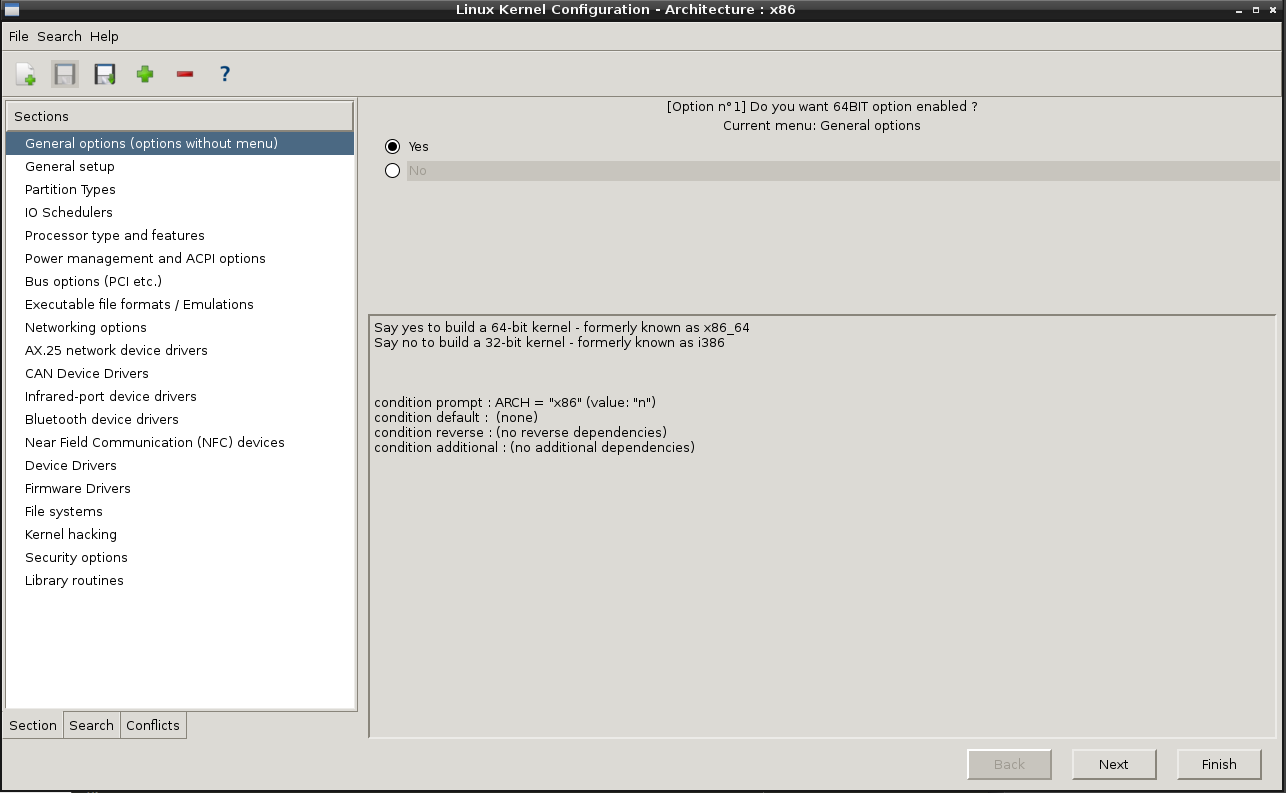
\includegraphics[scale=0.5]{./illustrations/screen_options_interface.png}
        \centering
        \caption{Évolution de l'interface d'affichage des options}
        \label{fig:Evo_config}
    \end{figure}

    Lorsqu'une option est sélectionnée, il n'y a plus seulement sa description
    d'affiché, mais également ses dépendances. Cela permet à l'utilisateur de 
    pouvoir corriger d'éventuels conflits plus facilement.

    \pagebreak  

    \item Évolution de l'interface de recherche des options
    \\

    L'onglet "Search" permet à l'utilisateur d'afficher la liste complète 
    des options sous la forme d'un arbre ou une liste plus réduite en 
    saisissant une chaine à rechercher.

    \begin{figure}[H]
        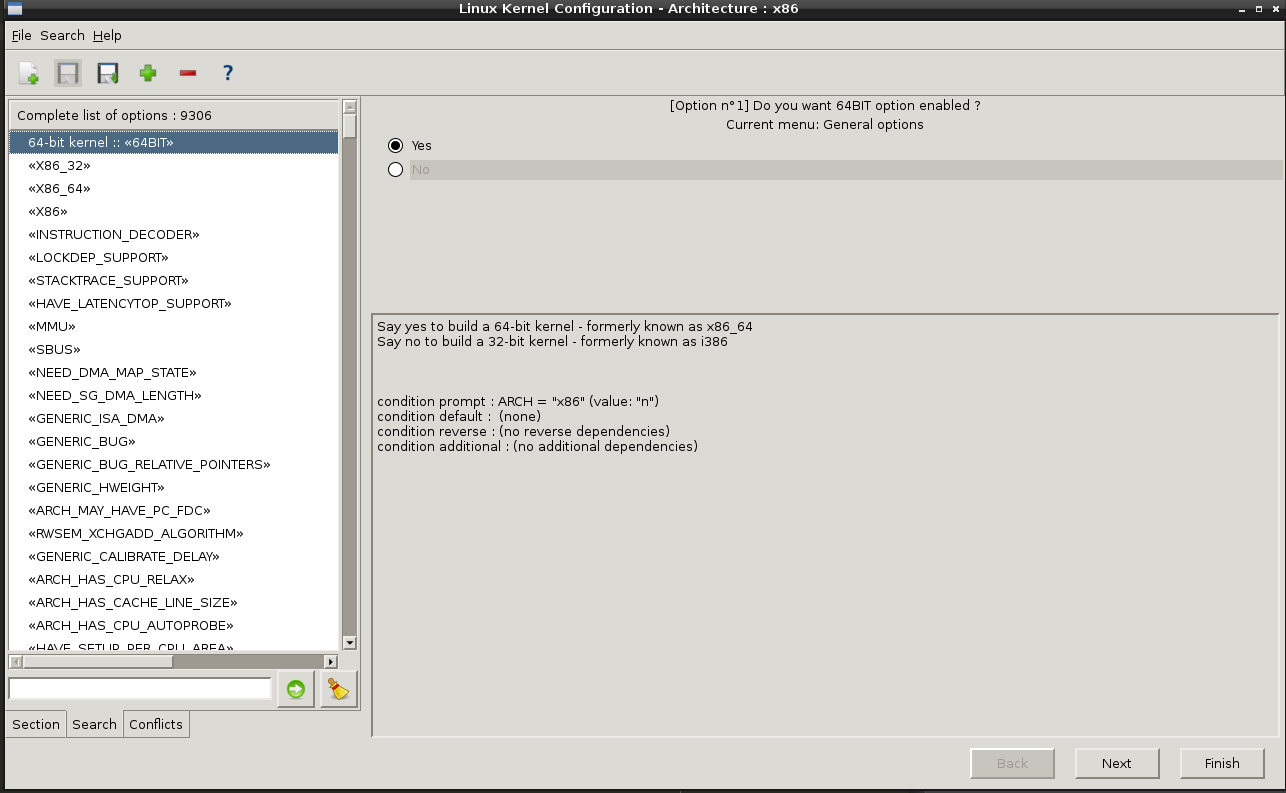
\includegraphics[scale=0.5]{./illustrations/screen_options_search_interface.png}
        \centering
        \caption{Évolution de l'interface de recherche des options}
        \label{fig:Evo_config}
    \end{figure}

    Dans les outils existants ainsi que dans les premiers prototypes, il est
    seulement possible de faire une recherche sur les noms des options. 
    Dorénavant, l'utilisateur peut cliquer le menu "Search" en haut de la 
    fenêtre pour sélectionner où il souhaite rechercher. Il peut chercher dans 
    les noms, les descriptions et les aides des options.
    \\

    \pagebreak  

    \item Évolution de l'interface d'affichage des conflits
    \\

    À l'origine, il y avait un bouton sur l'interface permettant d'ouvrir 
    une fenêtre pour résoudre les conflits. Il y avait un second bouton relatif 
    à l'ajout de Tags. Il a également disparu, car les tags sont uniquement 
    gérés par notre site.  


    \begin{figure}[H]
        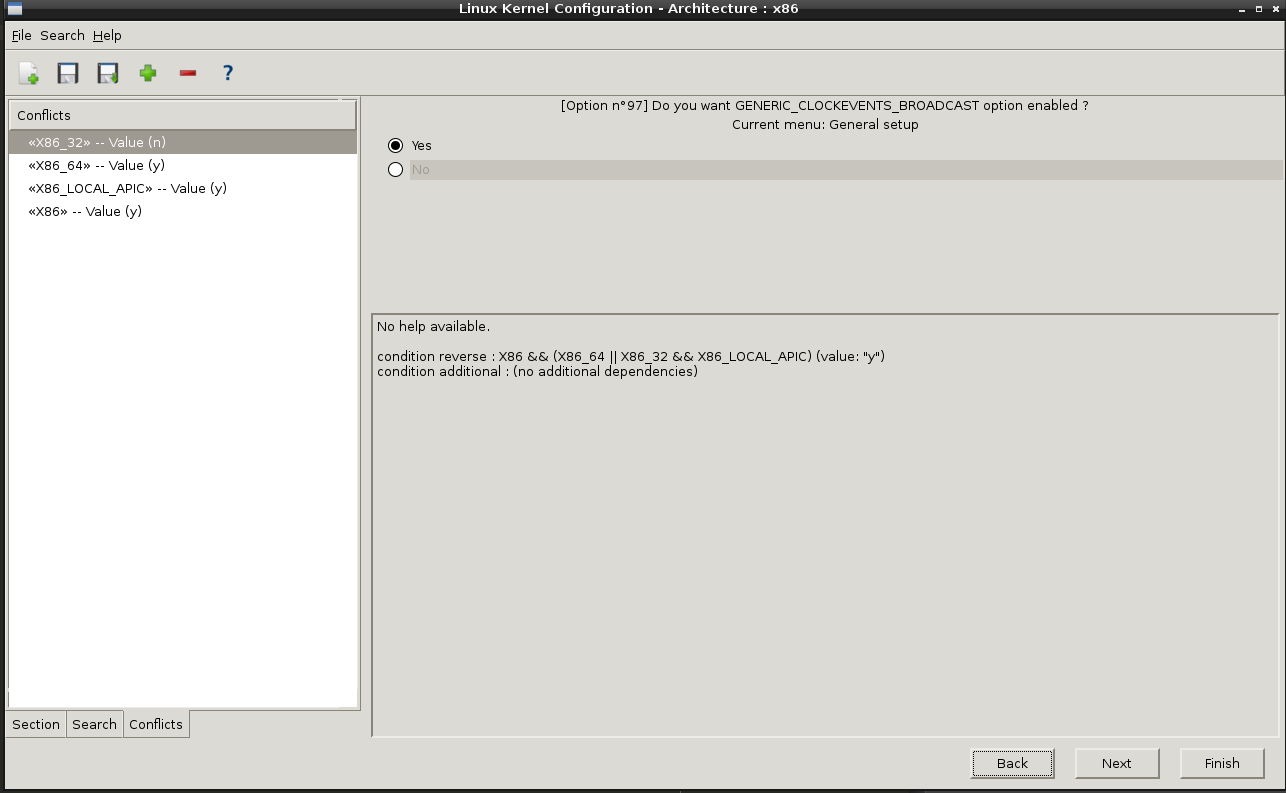
\includegraphics[scale=0.5]{./illustrations/screen_options_conflits_interface.png}
        \centering
        \caption{Évolution de l'interface d'affichage des conflits}
        \label{fig:Evo_config}
    \end{figure}

    Un nouvel onglet est apparu à droite de la recherche. L'idée de résoudre 
    les conflits automatiquement a été remplacée par cet onglet. Il affiche 
    la liste des options en conflit avec l'option courante. Cela permet à 
    l'utilisateur de se positionner rapidement sur les options qui posent 
    problème. 
    \\
\end{enumerate}

    \newpage
    \section{Site web}
    \label{sec:Site web}

    En réponse à l'évolution de nos besoins, nous avons conçu un site sous 
    la forme d'une base de données communautaires. A l'image du site 
    Wikipédia, les informations présentes sur ce site sont gérées par 
    les utilisateurs.\\

    En effet il est possible de : \\

    \begin{itemize}
        \item Ajouter des relations entre un matériel et un module
        \item Ajouter des relations entre une option et un module
        \item Ajouter des relations entre une option et un tag
        \item Supprimer ces relations
        \item Modifier ces relations
        \item Rechercher des relations existantes
    \end{itemize} 

    On peut voir ci-dessous la structure de la base de donnée du site. \\

    \begin{figure}[H]
        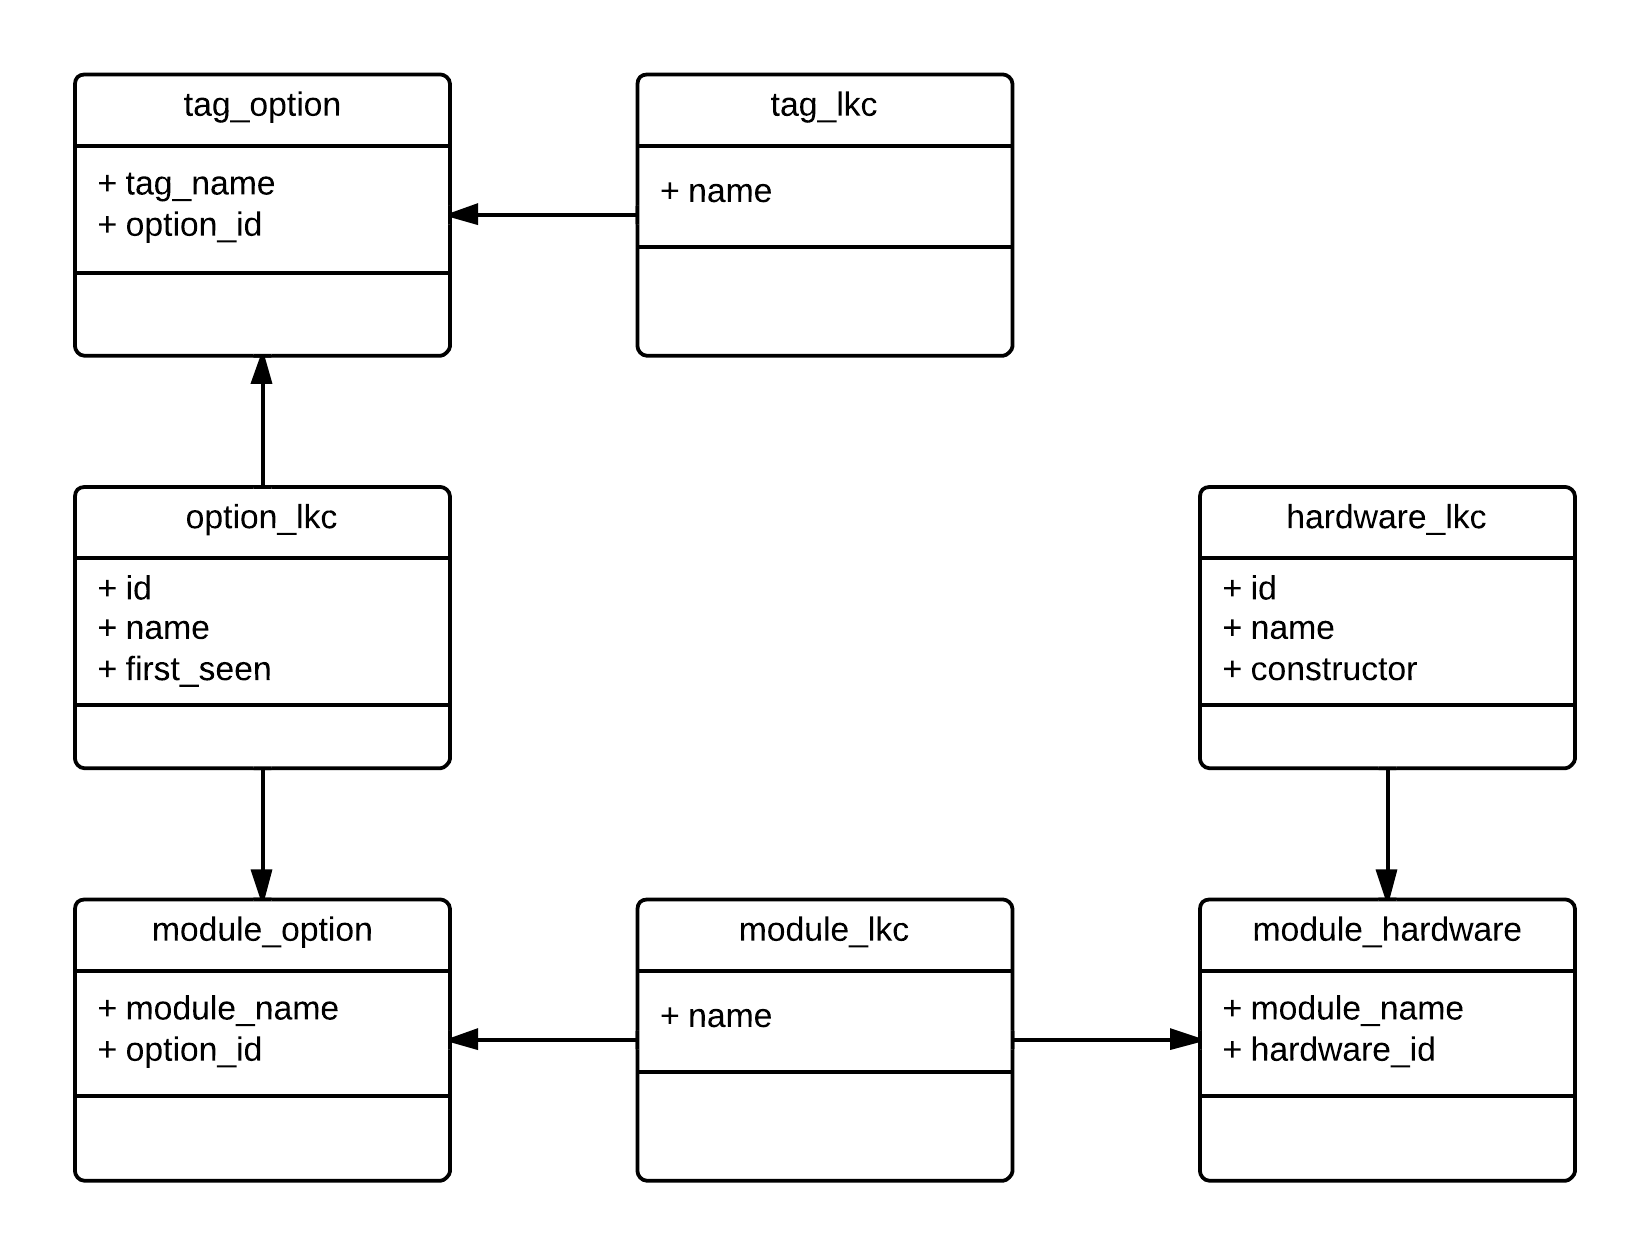
\includegraphics[scale=0.2]{./illustrations/diagramme_classes_site.png}
        \centering
        \caption{Diagramme des classes du site}
        \label{fig:DiagSite}
    \end{figure}


\chapter{Développement}
\label{cha:Développement}
    \section{Choix technologiques}
    \label{sub:Choix technologiques}

Dès les premières réunions avec notre client, nous avions discuté du langage à 
utiliser pour concevoir l'application. La première proposition était d'utiliser 
le langage C. En effet, vu que cette application a pour but d'être adoptée par 
la communauté Linux, il aurait été judicieux de la coder avec le langage 
qu'elle préfère. Dans un premier temps, nous avions pensé à la réaliser
en Java, mais ce langage n'est pas très apprécié par cette communauté.
\\

Ensuite, après avoir bien avancé dans la recherche de notre existant, nous 
avons trouvé une bibliothèque en Python permettant de manipuler les options 
d'un noyau Linux. Dans une optique d'homogénéité, nous avons décidé de réaliser 
toute notre application en Python et cela ne posait pas de problèmes au client.
\\

En ce qui concerne l'utilisation de la bibliothèque Python que nous avons 
trouvée, nous avions le choix entre refaire cette gestion nous-mêmes, ce qui 
aurait pris une grande partie de notre temps de développement et celui-ci 
était très limité. Nous avons donc décidé de nous servir de cet existant 
afin de pouvoir nous concentrer sur d'autres tâches comme l'affichage 
des options en conflits.


    \section{Architecture}
    \label{sub:Architecture}

Nous avons choisi de regrouper chacun de nos modules dans différents fichiers.
Au cours de notre développement, nous sommes passés par plusieurs approches
où nous n'avions pas pris en compte des éléments déjà existants pouvant être
réutilisés. Voici donc le résultat final.
\begin{figure}[H]
    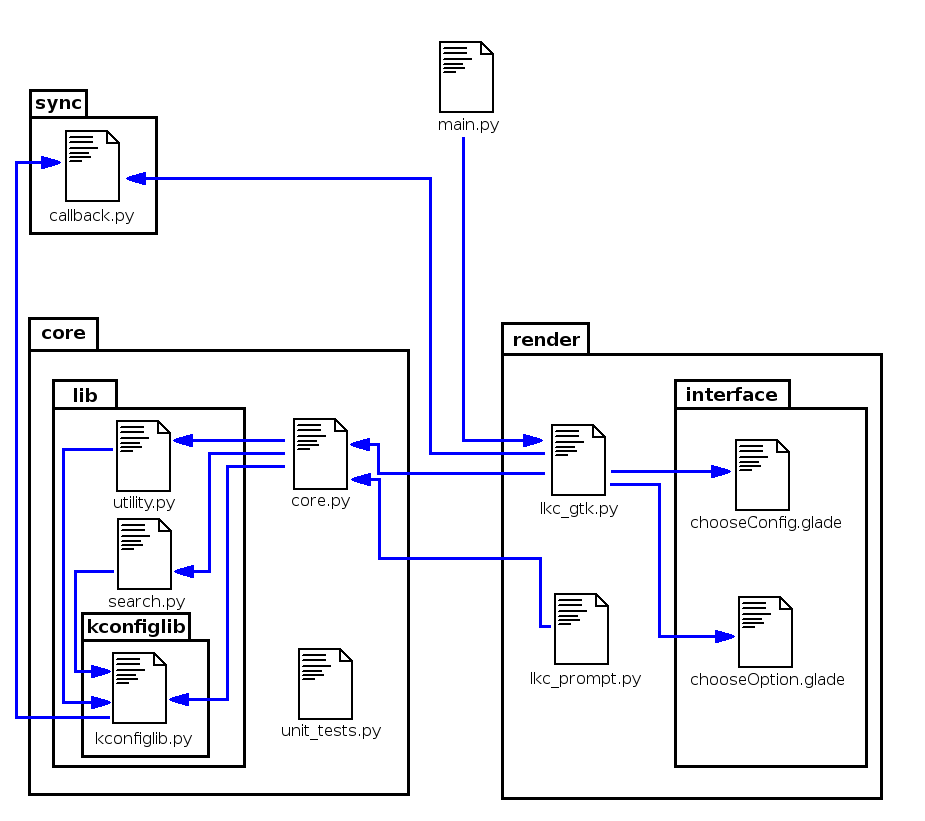
\includegraphics[scale=0.5]{illustrations/archi_add_v1.png}
    \centering
    \caption{Architecture}
    \label{fig:Arch}
\end{figure}

Les liaisons représentent les dépendances entre les différents fichiers.

\subsection{Décomposition modulaire}
\label{sec:Décomposition modulaire}
Notre architecture se base sur le design pattern MVVM (Model View
ViewModel) une variante du concept MVC. En effet, celui-ci contient une
partie de traitement centralisée dans le module core et son affichage dans
le module render.

La différence avec le modèle MVC (Model View Controller), c'est qu'il n'y a
pas de contrôleur.  La plupart du temps on l'utilise pour contraindre les
actions de l'utilisateur et n'avoir que des événements souhaités. Ce qui ne
nous a pas paru primordial dans notre projet.  Notre projet contient trois
modules principaux.

    \subsubsection{Core}
    \label{sub:Core}
    Le module core représente le \textit{modèle} de notre architecture.
    Celui-ci représente le coeur de notre application et contient
    ses principales caractéristiques.
    Il est utilisé pour l'initialisation, le parcours et le positionnement
    de valeurs d'options d'une configuration linux à générer. \\
    Ce module est lui-même décomposé en un sous-module utilisé comme
    bibliothèque interne. Celui-ci contient la bibliothèque kconfiglib, base
    de notre projet, ainsi que de deux modules utility et search nous
    permettant d'étendre les fonctionnalités de kconfiglib.
    Kconfiglib nous permet de charger en mémoire une configuration Linux
    pour une architecture donnée, modifier et d'en générer un fichier
    utilisable dans la compilation d'un noyau.
    L'utilisation de kconfiglib se fait principalement dans une arborescence
    d'un noyau Linux décompressé. Son exécution se fait à partir d'une cible
    de compilation afin de récupérer les variables d'environnement initialisées
    dans le Makefile principal du noyau Linux. \\
    Le module utility permet entre autres de faire "croire" à la bibliothèque
    kconfiglib que son exécution se fait bien dans à partir de cette cible en
    initialisant les variables d'environnement propres à son Makefile comme
    par exemple l'architecture choisie. \\
    Afin de récupérer les différentes conditions
    (prompt, default, select, reverse, additionnal) pour des pistes
    de résolutions de conflits, une idée était de parser le retour de la
    fonction \verb|__str__()| de chacun des \textit{symboles}.
    Cependant, kconfiglib avait déjà récupéré et mis en attribut des
    \textit{symboles} ces valeurs dans un format préfixe, sauf pour les
    dépendances additionnelles.\\
    Exemple pour l'option \verb|CONNECTOR|:
    \[\verb|[&&, [DM_MIRROR, NET, MD, DM_LOG_USERSPACE]|\\\]

    Sous cette forme, il est facile de créer un arbre qu'on puisse parcourir en
    profondeur pour ainsi avoir la notation infixe représentative.
    Chacun des noeuds auraient comme valeur soit un arbre, soit un opérateur
    logique (|| \&\& !) et au niveau des feuilles le nom d'un symbole.\\

    \begin{figure}[H]
        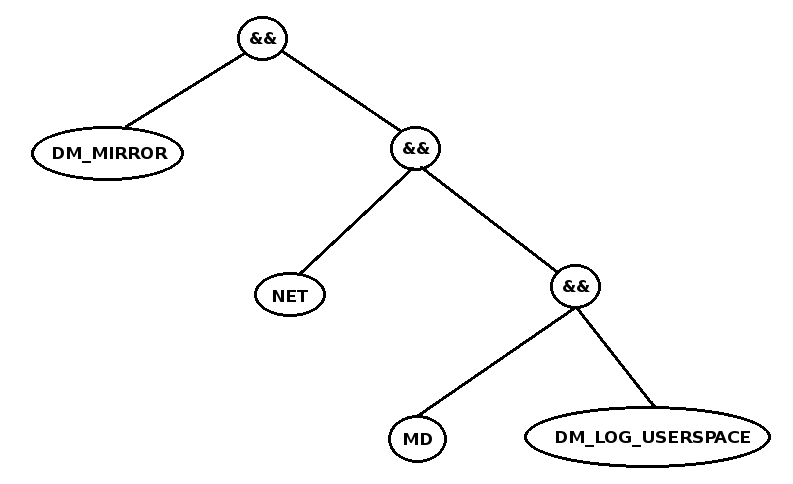
\includegraphics[scale=0.5]{illustrations/condition_tree.png}
        \centering
        \caption{Exemple d'une représentation en arbre d'une condition}
        \label{fig:condTree}
    \end{figure}

    Le module search, permet de chercher une liste d'options ayant au choix,
    dans leur nom, leur description, leur aide un mot-clé mis en entrée.

    \subsubsection{Render}
    \label{sub:Render}
    Le module render représente la \textit{vue} de notre architecture.
    Celui-ci représente l'interface visuelle du module core.
    Dans la version délivrée, il contient une implémentation GTK sous la forme
    de classes utilisant des fichiers XML générés avec l'outil Glade
    correspondant à nos maquettes.

    \subsubsection{Sync}
    \label{sub:Sync}
    L'architecture choisie rend l'application maintenable, modulaire et
    indépendante du choix de l'implémentation de l'IHM. En effet, la partie
    graphique ne fait qu'afficher l'état courant du \textit{modèle} et
    le module sync permet aux bibliothèques graphiques de mettre à jour un
    objet, tel qu'une barre de chargement. Ce mécanisme nous permet d'afficher
    l'avancement de l'initialisation du logiciel pour l'utilisateur final.
    \\
    
    De plus, le logiciel étant ouvert, on laisse à qui le souhaite le choix de
    modifier ou de changer le comportement proposé, mais aussi d'outil
    graphique. En effet, il est possible de migrer vers une autre solution
    telle que QT, pour un choix de portabilité avancé,  ou encore ncurses, ce
    qui répondrait à un de nos besoins non fonctionnel qui était de pouvoir
    lancer l'application en mode console sur un environnement avec ou sans
    serveur X.


    \section{Cycle de vie}
    \label{sub:Cycle de vie}

\begin{figure}[H]
    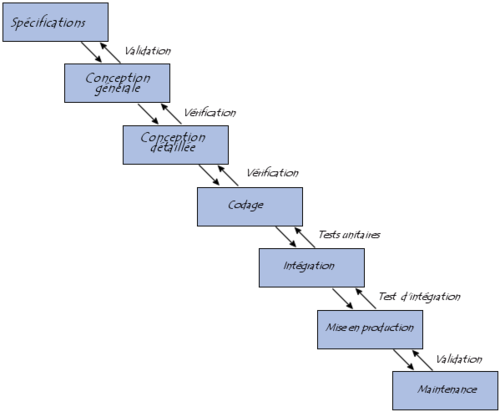
\includegraphics[scale=0.7]{./illustrations/cycle_cascade.png}
    \centering
    \caption{Schéma du cycle en cascade}
    \label{fig:CycleCascade}
\end{figure}

Ce projet a eu un cycle de vie en cascade avec retour. En effet, durant toutes 
les phases de notre projet, nous avons soumis notre travail à vérification 
et validation afin de pouvoir être en accord avec notre chargé de TD et notre 
client. L'utilisation de ce cycle de développement n'a pas été un choix, car 
il était imposé par le formalisme de cet enseignement. Cependant, celui-ci a 
été très utile, car il nous a permis de réaliser une analyse conséquente dès 
le début du projet afin de définir précisément les besoins de notre client.

\chapter{Tests effectués}
\label{cha:Tests}
    \section{Tests fonctionnels}
    \label{sec:Tests fonctionnels}

\subsection{Tests unitaires}

Pour les tests unitaires nous utilisons une API Python spécialisée dans les 
tests (unittest), toutes les fonctions dans la classe 
commençant par le mot « test » sont exécutes une par une.\\
\\
Pour essayer de rendre les tests homogènes, nous avons décidé de créer 3 
variables contenant les données nécessaires pour les tests :\\

\begin{itemize}
    \item Les paramètres passés à la fonction testée
    \item Le résultat attendu après le calcul de la fonction
    \item Le résultat après le calcul de la fonction
\end{itemize}

Une grande partie des fonctionnalités développées dans ce projet utilisent
des fonctions dont l'usage est assez générique (elles peuvent être utilisées
dans plein de cas différents et ne sont pas développées juste pour une 
fonctionnalité). Il est donc capital d'effectuer des tests sur ces fonctions
pour tenter de découvrir des comportements erronés ou inattendus.

Ces fonctions génériques sont dans le fichier application/modules/utility.py

\subsubsection{\texttt{test\_convert\_list\_xDim\_to\_1Dim}}

La fonction \verb|convert_list_xDim_to_1Dim| sert à 
convertir une liste à plusieurs dimensions en une liste d'une seule dimension.
\\
Exemple: [ [1,2] , [3] , [4 , [ 5 , 6 ] ] ] → [ 1 , 2 , 3 , 4 , 5 , 6 ]\\

Nous avons donc essayé de mettre en entrée des listes des tests complexes ou 
inhabituels, comme : \\

\begin{itemize}
    \item Une liste d’une dimension
    \item Une liste contenant des listes d'une grande profondeur
    \item Une liste contenant des listes vides
    \item Un autre objet qu'une liste
\end{itemize}

\subsubsection{\texttt{test\_convert\_tuple\_to\_list}}

Cette fonction sert à convertir un tuple en liste, elle est utile, car peu
d'opérations (intéressante pour nous) peuvent être effectuées sur les tuples, tout le contraire des 
listes. Il nous est donc plus aisé de travailler avec des listes, mais le 
plus souvent kconfiglib nous fournis des tuples. \\

Exemple: ( (1,2) , (3) , (4 , ( 5 , 6 ) ) ) → [ [1 , 2] , [3] , [4 , [5 , 6]]] 
\\

Les tests sont assez similaires à ceux de \verb|test_convert_list_xDim_to_1Dim|. \\


\subsubsection{\texttt{test\_get\_symbols\_list}}

Cette fonction permet de transformer un arbre représentant une condition
en une liste donnant le nom des symboles (options) présents dans cette 
condition. Le principe derrière ce test et de vérifier qu'on récupère
uniquement les options, on ne désire pas avoir les autres objets 
de la condition (comme des opérateurs booléens) dans la liste.
Il est à noter que la fonction est susceptible de retourner une liste dont 
certain élément seraient des éléments booléens (y,n) ou tristate (y,n,m). 
Mais un traitement ultérieur (hors de la fonction) est fait pour épurer le résultat (on ne 
veut vraiment que le nom des symboles).\\

Cette fois le but du test était vraiment de tester la fonction avec des 
conditions assez complexes. Il est important de préciser qu'une grande 
majorité des cas d'erreur est directement géré dans la fonction elle-même.\\

Le test de cette fonction à l'avantage de tester une nouvelle fois la 
fonction \verb|convert_list_xDim_to_1Dim|.

\subsubsection{\texttt{test\_get\_first\_option\_menu}}

Ce test vérifie que la première option d'un menu est définie par un indice
plus grand que -2 et moins grand que le nombre total d'option

\subsubsection{\texttt{test\_get\_index\_menu\_option}}

Dans l'onglet section de notre application, nous affichons une liste des 
menus se trouvant en haut de l'arborescence. C'est à dire que nous n'affichons 
aucun menus qui sont dans des menus. Lorsque l'utilisateur navigue dans les 
options nous mettons en surbrillance le menu dans lequel se trouve l'option. 
Ce test permet de vérifier la plage des valeurs de retour de la fonction. 
Si la fonction renvoie 0 c'est que l'option ne se trouve pas dans un menu 
sinon la fonction renvoie l'indice du menu oû se trouve l'option. Cette 
indice atteint au maximum le nombre de menus de haut niveau.

\subsubsection{\texttt{test\_get\_all\_items}}

Cette fonction permet de convertir le résultat d'une autre fonction 
"get\_top\_level\_items()" qui retourne la liste des items de haut niveau. 
C'est à dire que cette fonction parcours l'ensemble des options en mémoire 
et lorsqu'elle tombe sur un "Menu" par exemple, elle le retourne plutôt que 
de retourner les options qui sont à l'intérieur. La fonction 
"get\_all\_items()" permet de récupérer uniquement les options et les choix 
en parcourant en profondeur tous les items. Les menus et les commentaires 
sont enlevés par cette fonction. Ce test vérifie qu'il ne reste plus que 
des "symbols" et des "choice" dans la liste retournée.


\subsubsection{Test parcours de la liste des options}

Ce n'est pas vraiment un test unitaire, mais le fait de parcourir 
automatiquement la liste de toutes les options nous permet de savoir rapidement,
pour chaque option, si les fonctions gérant l'affichage ne contiennent pas 
d'erreur.
\\

Le test simule l'appui sur le bouton next par l'utilisateur jusqu'à ce qu'il
arrive à la fin de la liste des options. On peut donc rapidement détecter si 
une erreur est présente sans devoir faire défiler les options une par une 
nous-mêmes. Ce test a été mis en place suite aux erreurs découvertes lors de
l'affichage de certaines options afin de tenter de toutes les détecter et de 
toutes les corriger.


    \section{Tests non fonctionnels}
    \label{sec:Tests non fonctionnels}

\subsection{Fuite de mémoire}

Nous avons utilisé un outil (smem), couplé à un script, pour consulter la 
mémoire utilisée par notre application à n'importe quel moment. Nous avons 
donc tenté de suivre l'évolution de la mémoire après certaines actions supposées
fréquentes de l'utilisateur :

\begin{enumerate}
    \item Sauvegarde d'une configuration : Nous avons remarqué que 
          plusieurs sauvegardes à la suite entrainent une consommation 
          (non excessive) de la mémoire, mais elle semble redescendre
          peu de temps après au niveau initial.

    \item Défilement des options : Le défilement des options n'entraine
          aucune fuite mémoire.
    \item Recherche : La recherche n'entraine aucune fuite mémoire.
\end{enumerate}


\subsection{Tests de portabilité}

Une des demandes du client était que notre application réponde à la contraite
de la portabilité. Étant donné que nous avons utilisé python (qui peut être 
exécuté sur les plateformes Linux, Mac, Windows), nous avons raisonnablement
pensé que notre application fonctionnerait sur ces trois plateformes et les tests
ont témoigné de son fonctionnement. L'aspect de l'interface graphique semble
subir de légères modifications selon si l'application est exécutée sur Linux,
Mac ou Windows, mais nous n'avons pas jugé ces différences comme étant
problématique pour l'utilisateur.\\

Note : Pour l'utilisation de notre application sur Windows, il a fallu modifier
très légèrement l'api kconfiglib. En effet, celle-ci utilisait la fonction
os.uname() qui n'est présente que dans les systèmes unix, par conséquent, nous
avons commenté cette ligne dans le code, puisque nous n'utilisons jamais cette 
fonctionnalité.

\subsection{Vitesse au chargement}

Les performances ne sont pas forcément importante pour ce genre d'application,
mais nous avons tout de même voulu voir la comparaison des vitesses au 
chargement du noyaux entre notre application et les outils existant:\\

Nous avons fait cinq tests pour chaque application:\\

%TODO mieux commenter le schéma

\begin{tabular}{|c|c|}
\hline
test LKC & temps (en sec) \\
\hline
\hline
1 & 11.56 \\
\hline
2 & 13.67 \\
\hline
3 & 9.13 \\
\hline
4 & 10.56 \\
\hline
5 & 12.80 \\
\hline
\end{tabular}
\newline
\newline

\begin{tabular}{|c|c|}
\hline
test XCONFIG & temps (en sec) \\
\hline
\hline
1 & 18.42 \\
\hline
2 & 15.03 \\
\hline
3 & 18.94 \\
\hline
4 & 12.23 \\
\hline
5 & 21.10 \\
\hline
\end{tabular}
\newline
\newline

\begin{tabular}{|c|c|}
\hline
test GCONFIG & temps (en sec) \\
\hline
\hline
1 &  9.77 \\
\hline 
2 & 9.31 \\
\hline
3 & 7.18 \\
\hline
4 & 11.42 \\
\hline
5 & 8.78 \\
\hline
\end{tabular}

\begin{figure}[H]
    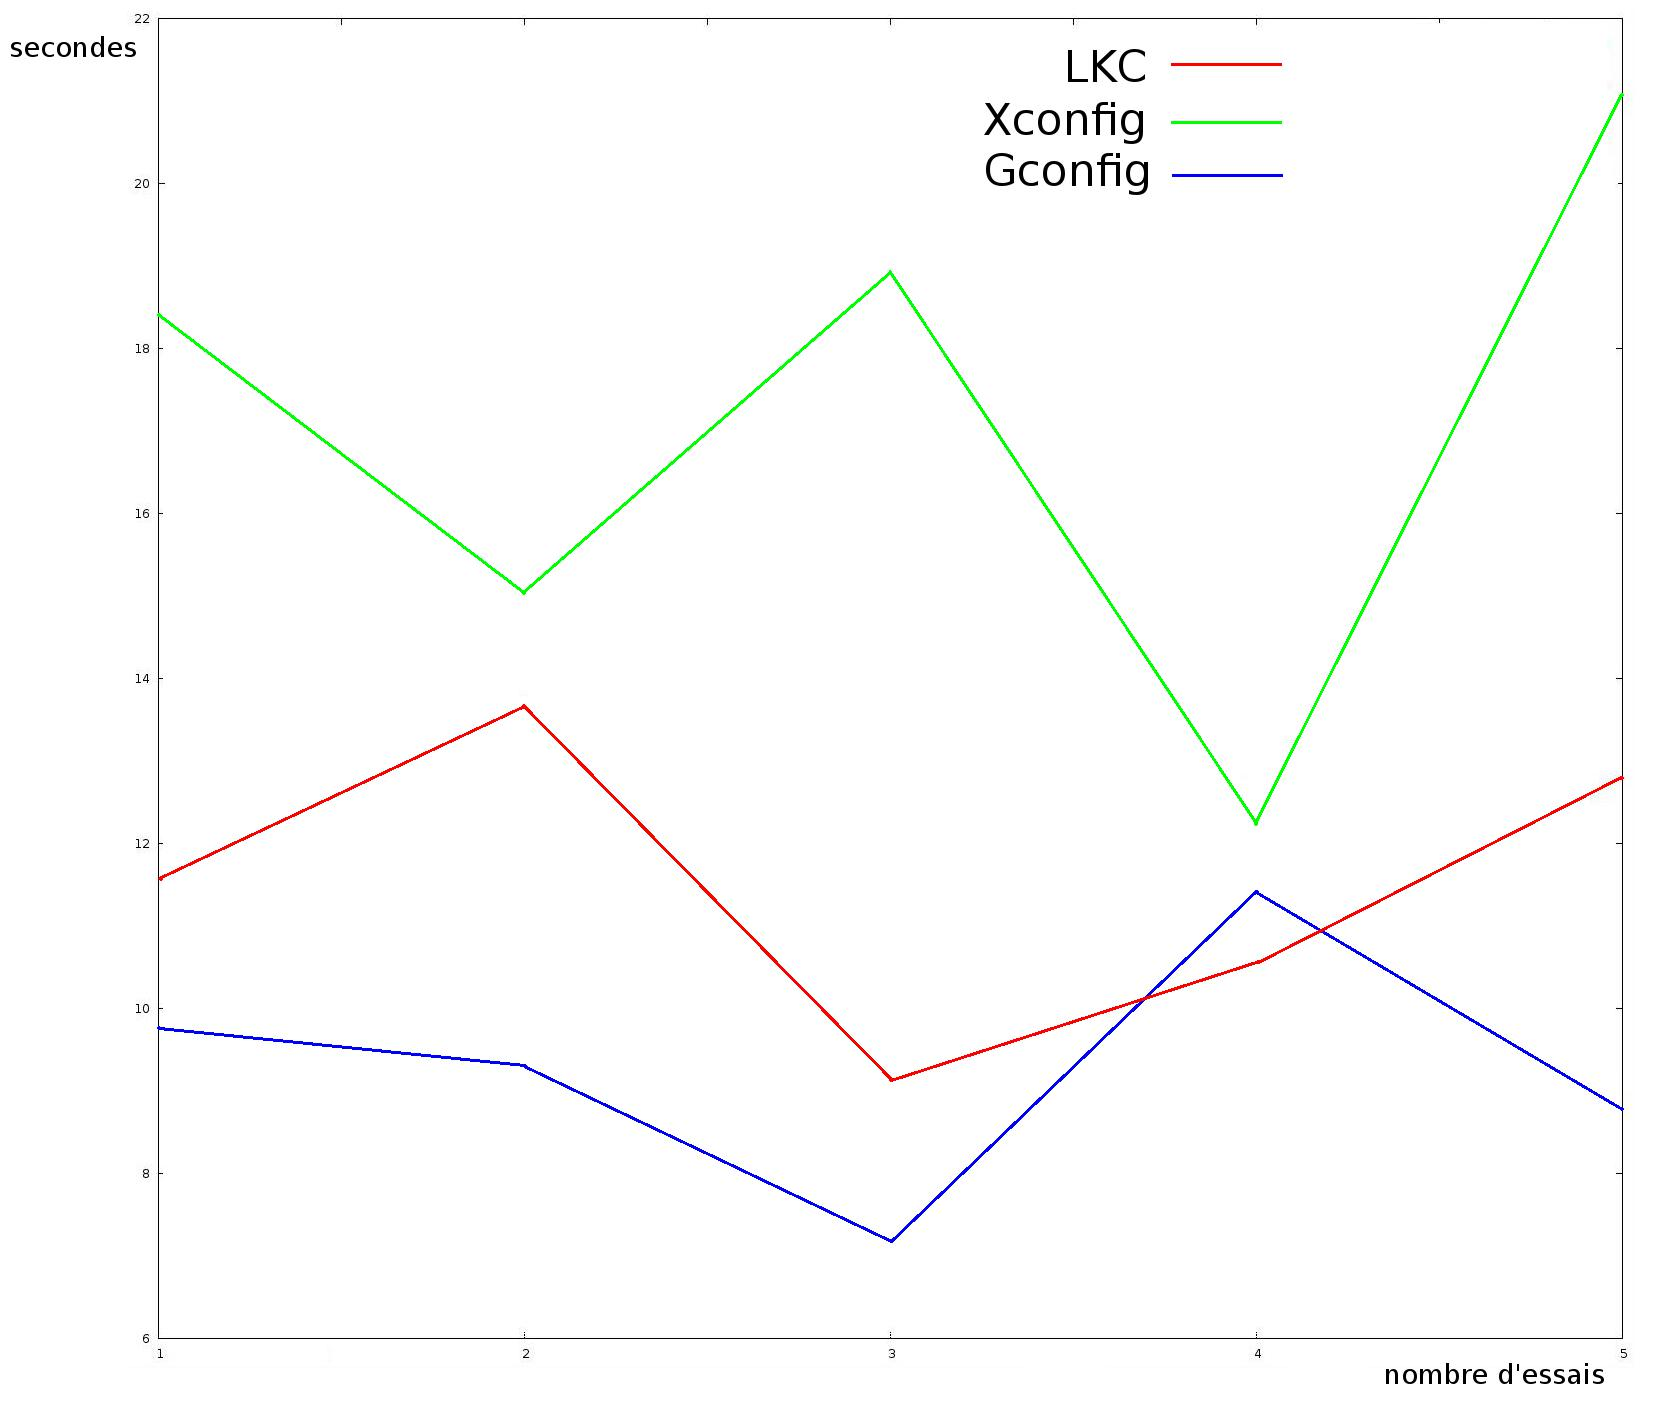
\includegraphics[scale=0.5]{./illustrations/speed_cmp.jpeg}
    \centering
    \caption{Comparaison des vitesses de chargement des noyaux}
    \label{fig:VitesseChargement}
\end{figure}


\chapter{Résultats}
\label{cha:Résultats}
    \section{Ce qui a été fait}
    \label{sec:Ce qui a été fait}
    % === TODO ===
    %Logiciel : TODO

    Par rapport aux outils existants, il est possible de visualiser les options
    qui ne sont pas modifiables, et ainsi savoir pourquoi elle ne le sont pas.
    Il est de plus possible d'accéder aux options posant problème afin d'essayer
    de satisfaire les multiples conditions présentes pour une option donnée.

    Nous avons développé un site à but communautaire pour l'obtention d'information
    sur le matériel compatible avec des options associées à un noyau Linux. Ce site
    permet également de catégoriser des options à partir des mots-clés.

    \section{Ce qui reste à faire}
    \label{sec:Ce qui reste à faire}
    Il faudrait mieux catégoriser les sections pour des utilisateurs non-experts.
    En effet, actuellement on récupère les menus racines des fichiers Kconfig,
    alors que nous pourrions créer nos propres groupes d'options, ce qui pourrait
    être plus précis et plus pertinent. Cependant, ce tri peut être sujet à l'erreur
    par manque d'information et peut aussi être difficile à réaliser.

    %TODO Bison/Lex
    Étant bloqué dans le choix du langage de programmation avec la bibliothèque
    utilisée, kconfiglib, on pourrait éventuellement réfléchir à une alternative
    pour un chargement plus rapide en mémoire d'une configuration Linux.

    A court terme, la fonctionnalité la plus importante à ajouter
    à notre application serait de créer une correspondance entre la base de donnée du
    site communautaire et l'application. Grâce à ça, il serait possible de faire des
    recherches d'options par rapport à un nom de matériel, au sein même de la
    recherche. On pourrait également rechercher des options en fonctions des
    tags que la communauté aura crée. Au fil du temps, les données du site
    s'affineront pour être de plus en plus précis. On peut également
    imager que d'autres informations seront modifiable à partir du site,
    comme la description des options.

    Avoir une réelle gestion du site communautaire, avec vérification des entrées.
    Rajouter une option afin de visualiser les options qui ne sont pas modifiable
        telles que les options STRING/HEX/INT.

    Il serait également possible de pousser encore plus loin l'aspect portabilité.
    En effet, via le site, on pourrait laisser la possibilité de configurer un
    noyau Linux.

    Afin d'aider l'utilisateur final dans sa résolution de conflits, on peut
    envisager une résolution automatique des conflits de manière sommaire
    \textit{"Get lucky"}.  Afin de ne pas trop prendre de temps dans les
    essais, on pourrait éventuellement restreindre le niveau de profondeur du
    parcours des dépendances d'une option.

\chapter{Conclusion et bilan}
\label{cha:Conclusion et bilan}

Ce projet de programmation a été l'aboutissement de notre première année 
de Master Informatique à l'université de Bordeaux. Celui-ci nous a apporté 
beaucoup en ce qui concerne l'expérience de la réalisation d'un projet 
informatique dans son ensemble et il a également été bénéfique au niveau 
technique et relationnel.\\

Dans un premier temps, au niveau technique, ce projet nous a permis 
d'approfondir nos compétences dans certains langages que nous avions 
précédemment utilisé comme le Python, mais aussi d'en apprendre de 
nouveaux comme GTK pour réaliser la partie graphique. Nous avons ainsi 
élargi nos connaissances informatiques. Nous avons du nous familiariser 
avec la bibliothèque "Kconfiglig" pour intéragir avec les options d'un 
noyau Linux. De même, nous avons pu constater l'importance de l'analyse 
et conception dans un projet concret, en nous permettant de fixer les bases 
du projet afin d'avoir des documents sur lesquels s'appuyer. Ils seront 
d'autant plus utiles aux personnes qui voudraient reprendre notre projet 
dans l'avenir.\\

Dans un second temps, concernant l'aspect relationnel, nous avons beaucoup 
appris, qu'il s'agisse de la communication interne au groupe, ou de la 
communication avec l'extérieur. Il a été nécessaire de comprendre et de 
détailler les différents besoins de nos commanditaires. Cette étape nous 
a pris beaucoup de temps, mais nous a permis d'avoir des documents d'analyse 
détaillés pour réaliser la partie technique de manière plus fluide et efficace. 
Ensuite, nous avons pu travailler en groupe sur tout un semestre. Nous 
avons pu ainsi nous rendre compte qu'il n'est pas toujours évident de gérer 
une équipe avec les tensions qui peuvent apparaître. Mais nous avons réussi à 
réaliser ce travail en répartissant les tâches à accomplir et en nous 
réunissant fréquemment pour tenir compte des problèmes rencontrés.\\


\chapter{Annexes}
\label{cha:Annexes}
    \section{Documentation / manuel}
    \label{sec:Documentation / manuel}
    % === TODO ===

\bibliography{./bibliographie}
\end{document}
